\documentclass[12pt, a4paper, headinclude, twoside, plainheadsepline, open=right, numbers=noenddot, hidelinks, toc=listof, toc=bibliography]{scrreprt}

%&pdflatex

%\usepackage{showframe}


% WICHTIG: Hier wird nicht BibTeX sondern BibLateX verwendet!!
% Deshalb nicht mit bibtex uebersetzen, sondern mit biber
% Das kann man in jedem Tool wie TexMaker oder TexShop als Option einstellen
%
%% Spezielle Einstellungen, insbesondere fuer das Literaturverzeichnis,
% aber auch Packages wie amsmath, Groessenanpassungen etc.
%%%%%%%%%%%%%%%%%%%%%%%%%%%%%%%%%%%%%%%%%%%%%%%%%%%%%%%%%%%
% Allgemeines
\usepackage[automark]{scrlayer-scrpage}	% Kopf- und Fusszeilen
\usepackage{hyperref} 					% Internetseiten
\usepackage{acro}		% Abkuerzungen					
%\usepackage{showframe}


\acsetup{list/display=all}

%%%%%%%%%%%%%%%%%%%%%%%%%%%%%%%%%%%%%%%%%%%%%%%%%%%%%%%%%%%
% Encoding 
\usepackage[T1]{fontenc}
\usepackage{lmodern}
\usepackage[utf8]{inputenc} 							% UTF8-Kodierung fuer Umlaute usw
\usepackage[english]{babel}								% Deutsche Rechtschreibung
\RequirePackage[ngerman=ngerman-x-latest]{hyphsubst}	% Silbentrennung
\usepackage{csquotes}
\usepackage{microtype,textcomp}		


%%%%%%%%%%%%%%%%%%%%%%%%%%%%%%%%%%%%%%%%%%%%%%%%%%%%%%%%%%%
% Bildunterschrift
\usepackage[font=small,
			labelfont=bf]{caption}		% Formatierung von captions
			
\setcapindent{0em} 						% kein Einruecken der Caption von Figures und Tabellen
\setcapwidth{0.9\textwidth}
\setlength{\abovecaptionskip}{0.2cm} 	% Abstand der zwischen Bild- und Bildunterschrift
\captionsetup[table]{justification=justified,singlelinecheck=false,margin={-0cm,0cm}}
\captionsetup[subfigure]{oneside,margin={-0cm,0cm}}
\captionsetup[algorithm]{labelsep=colon,justification=justified,singlelinecheck=false,margin={-0cm,0cm}}

\usepackage{float}
\floatstyle{plaintop}
\restylefloat{algorithm}


%%%%%%%%%%%%%%%%%%%%%%%%%%%%%%%%%%%%%%%%%%%%%%%%%%%%%%%%%%%
% Mathematik
\usepackage{amsmath} 
\usepackage{amsfonts}
\usepackage{amssymb}


% \usepackage[locale=DE,
% 			group-four-digits,
%        		group-digits=integer,
% 			group-separator=.,
% 			detect-weight=true, 
% 			detect-family=true,
% 			]{siunitx}  			% SI Einheiten



%%%%%%%%%%%%%%%%%%%%%%%%%%%%%%%%%%%%%%%%%%%%%%%%%%%%%%%%%%%
% Tabellen
\usepackage{multirow} 	% Tabellen-Zellen ueber mehrere Zeilen
\usepackage{multicol} 	% mehre Spalten auf eine Seite
\usepackage{tabularx} 	% Fuer Tabellen mit vorgegeben Groessen
\usepackage{longtable}	% Ausrichtung des Abkürzungsverzeichnisses
\usepackage{rotating}	% Gedrehte Tabellen (sidewaystable)
\usepackage{colortbl} 	% Farbe für Zelle
\usepackage{ragged2e}	% Rechtsbündige P Spalte


\newcolumntype{R}[1]{>{\RaggedLeft\arraybackslash}p{#1}} % Rechtspündige p Spalte (feste Breite)


%%%%%%%%%%%%%%%%%%%%%%%%%%%%%%%%%%%%%%%%%%%%%%%%%%%%%%%%%%%
% Bilder
\usepackage{graphicx} 				% Bilder
\usepackage{epstopdf} 				% enable eps graphics
\usepackage{subfig} 				% mehrere Abbildungen nebeneinander/uebereinander
\usepackage{xcolor} 				% Farben
\usepackage[export]{adjustbox}		% Rahmen fuer Bilder (cframe=lightgray)



%%%%%%%%%%%%%%%%%%%%%%%%%%%%%%%%%%%%%%%%%%%%%%%%%%%%%%%%%%%
% Quellcode
\usepackage{listings} 					% fuer Formatierung in Quelltexten
\usepackage{scrhack}  					% removes Warning: \float@addtolists detected!  Caused by package listings
\usepackage[final,outer]{struktex} 	  	% Struktugramme
\usepackage[plain]{algorithm}
\usepackage[noend]{algpseudocode} 		% pseudo code


%%%%%%%%%%%%%%%%%%%%%%%%%%%%%%%%%%%%%%%%%%%%%%%%%%%%%%%%%%%
% Zeichnungen/Plots
\usepackage{pgfplots}						% Plots
\usetikzlibrary{matrix}						% Matrizen zeichnen
\usepackage{tikz}							% tikz picture
\usepackage{tikz-qtree,tikz-qtree-compat}	% Bäume
\usepackage{dirtree}						% Dateistrukutr

\pgfplotsset{compat=1.15}

%%%%%%%%%%%%%%%%%%%%%%%%%%%%%%%%%%%%%%%%%%%%%%%%%%%%%%%%%%%
% Sonstiges:
% Durchgehende Nummerierung. Ohne Chapter
\usepackage{chngcntr}
\counterwithout{equation}{chapter}
\counterwithout{figure}{chapter}
\counterwithout{table}{chapter}



%%%%%%%%%%%%%%%%%%%%%%%%%%%%%%%%%%%%%%%%%%%%%%%%%%%%%%%%%%%
%
% Einstellungen zum Literaturverzeichnis
%
% Hier eine von zwei Varianten auswaehlen: Nummern oder Buchstaben fuer Referenzen
%
%\usepackage[backend=biber, style=alphabetic, sorting=nyt]{biblatex}
\usepackage[
	backend=biber, 
	style=numeric-comp, 
	sorting=none,
	backref=true,
	backrefstyle=three+
	]{biblatex}
	
	
\ExecuteBibliographyOptions{%
     maxbibnames=99,   % Alle Autoren (kein et al.)
     maxcitenames=1,   % Kuerzel nur aus 1. Autor im Text
     maxalphanames=1,  % nur 1. Autor in der Abkuerzung
     backref=false,    % keine Ruueckverweise auf Zitatseiten
     giveninits=true,  % Vornamen abkuerzen
     isbn=false,       % ISBN ausblenden
     doi=false,        % DOI ausblenden
   }
   
   
\DefineBibliographyStrings{english}{
   andothers = {{et\,al\adddot}},            
} 
   
   
\renewcommand*{\labelalphaothers}{} % alpha label ohne +
%
\renewbibmacro*{volume+number+eid}{%
     \setunit{\space}\printfield{volume}%
     \iffieldundef{number}{}{%
      \printtext[parens]{\printfield{number}}}%
     \setunit{\addcomma\space}\printfield{eid}}
%
% no word 'pages' for articles in the bibliography (print as is)
\DeclareFieldFormat[article, inproceedings, incollection, unpublished]{pages}{#1} 
% no quotes for article titles (print as is)
\DeclareFieldFormat[article, inproceedings, incollection, online, unpublished]{title}{#1} 
%
\renewbibmacro*{date}{\printdate}
\renewbibmacro*{issue+date}{\usebibmacro{issue}}
\renewbibmacro*{publisher+location+date}{\printlist{publisher}}
%
   \setcounter{biburlnumpenalty}{9000}
   \setcounter{biburlucpenalty}{9000}
   \setcounter{biburllcpenalty}{9999}
%
% "In:" removed for articles; issue/date macros added after note+pages macro
\DeclareBibliographyDriver{article}{%
  \usebibmacro{bibindex}%
  \usebibmacro{begentry}%
  \usebibmacro{author/translator+others}%
  \setunit{\labelnamepunct}\newblock%
  \usebibmacro{title}%
  \newunit%
  \printlist{language}%
  \newunit\newblock%
  \usebibmacro{byauthor}%
  \newunit\newblock%
  \usebibmacro{bytranslator+others}%
  \newunit\newblock%
  \printfield{version}%
  \newunit\newblock%
  \usebibmacro{journal+issuetitle}%
  \newunit%
  \usebibmacro{byeditor+others}%
  \newunit%
  \usebibmacro{note+pages}%
  \setunit{\addcomma\addspace}%
  \usebibmacro{date}%
  \usebibmacro{finentry}}
%
%
\DeclareBibliographyDriver{inproceedings}{%
    \usebibmacro{begentry}%
    \printnames{author}%
    \setunit{\labelnamepunct}\newblock%
    \printfield{title}%
    \setunit{\labelnamepunct}%
	\usebibmacro{in:}%    
    \newblock%
    \ifnameundef{editor}%
    {%
    		\setunit{\adddot\space}%
    		\newunit%
    }%
    {%
     	\setunit{\addspace}%
     	\printnames[byeditor]{editor}%
     	\clearname{editor}%
     	\setunit{\space}%
     	\printtext[parens]{Hrsg.}%
     	\setunit{\addcolon\space}%
     	\newunit%
     }%
	\printfield{booktitle}%
	\setunit{\addcomma\space}%
	\printfield{pages}%
	\setunit{\addcomma\space}%
    \usebibmacro{date}%
    \usebibmacro{finentry}
}

\DeclareBibliographyDriver{book}{%
  \usebibmacro{bibindex}%
  \usebibmacro{begentry}%
  \usebibmacro{author/editor+others/translator+others}%
  \setunit{\labelnamepunct}\newblock
  \usebibmacro{maintitle+title}%
  \newunit
  \printlist{language}%
  \newunit\newblock
  \usebibmacro{byauthor}%
  \newunit\newblock
  \usebibmacro{byeditor+others}%
  \newunit\newblock
  \printfield{edition}%
  \newunit
  \iffieldundef{maintitle}
    {\printfield{volume}%
     \printfield{part}}
    {}%
  \newunit
  \printfield{volumes}%
  \newunit\newblock
  \usebibmacro{series+number}%
  \newunit\newblock
  \printfield{note}%
  \newunit\newblock
  \usebibmacro{publisher+location+date}%
  \newunit\newblock
  \usebibmacro{chapter+pages}%
  \newunit
  \printfield{pagetotal}%
  \newunit\newblock
  \usebibmacro{doi+eprint+url}%
  \newunit\newblock
  \usebibmacro{addendum+pubstate}%
  \setunit{\bibpagerefpunct}\newblock
  \usebibmacro{pageref}%
  \setunit{\addcomma\space}
  \usebibmacro{date}
  \usebibmacro{finentry}}
%  
%
 \DeclareBibliographyDriver{online}{%
   \usebibmacro{bibindex}%
   \usebibmacro{begentry}%
   \ifnameundef{author}
    {\printtext{Autor unbekannt}}
    {
		\usebibmacro{author/editor+others/translator+others}%    
    }%
   \setunit{\labelnamepunct}\newblock
   \usebibmacro{title}%
   \newunitpunct
   \usebibmacro{url+urldate}%
   %\usebibmacro{addendum+pubstate}%
   \usebibmacro{finentry}}  
%%%%%%%%%%%%%%%%%%%%%%%%%%%%%%%%%%%%%%%%%%%%%%%%%%%%%%%%%%%






%%%%%%%%%%%%%%%%%%%%%%%%%%%%%%%%%%%%%%%%%%%%%%%%%%%%%%%%%%%
% Eigene Befehle 
% Matrix
\newcommand{\mat}[1]{
      {\textbf{#1}}
}
\newcommand{\todobox}[1]{
      {\colorbox{red}{ TODO: #1 }}
}
\newcommand{\todo}[1]{
      {\color{red}{ TODO: #1}} \normalfont
}
\newcommand{\info}[1]{
      ({\color{blue}{INFO: #1}}\normalfont)
}
\newcommand{\code}[1]{
      {\ttfamily{#1}}
}


\usepackage{suffix}		%newcommand with suffix (*)
% Referenzierung auf subfigures 
\newcommand\sref[1]{\protect\subref{#1}}
\WithSuffix\newcommand\sref*[1]{\protect\subref*{#1}}


% Mathematik-Operatoren
\DeclareMathOperator{\atantwo}{atan2}





%%%%%%%%%%%%%%%%%%%%%%%%%%%%%%%%%%%%%%%%%%%%%%%%%%%%%%
% Deutsche Begriffe fuer Pseudocode (algorithm)
%
\floatname{algorithm}{Algorithm}
\renewcommand{\algorithmicrepeat}{\textbf{repeat}} 
\renewcommand{\algorithmicuntil}{\textbf{until}} 
\renewcommand{\algorithmicfor}{\textbf{for}} 
\renewcommand{\algorithmicend}{\textbf{}} 
\renewcommand{\algorithmicdo}{} 

\algnewcommand\algorithmicforeach{\textbf{for each}}
\algdef{S}[FOR]{ForEach}[1]{\algorithmicforeach\ #1\ \algorithmicdo}






%%%%%%%%%%%%%%%%%%%%%%%%%%%%%%%%%%%%%%%%%%%%%%%%%%%%%%
% Groessenanpassungen
%
\setlength{\unitlength}{1cm}
\setlength{\oddsidemargin}{0.3cm}
\setlength{\evensidemargin}{0.3cm}
\setlength{\textwidth}{15.5cm}
\setlength{\topmargin}{-1.2cm}
\setlength{\textheight}{23cm}
\columnsep 0.5cm


%%%%%%%%%%%%%%%%%%%%%%%%%%%%%%%%%%%%%%%%%%%%%%%%%%%%%%
% Silbentrennung
%
\hyphenation{Über-le-bens-wahr-schein-lich-keit}

\usepackage{placeins}


%

% Hier werden die Referenzen in einer separaten Datei gespeichert
\addbibresource{Thesis.bib}
%
%%%%%%%%%%%%%%%%%%%%%%%%%%%%%%%%%%%%%%%%%%%%%%%%%%%%%%%%%%%%%

%----------------------------------------------------------------------------------
%  Informationen
%----------------------------------------------------------------------------------
\author{Maximilian Rieder}
\title{Robust Segmentation in Minimally Invasive Surgery for Smoke Interference}
\date{\today}


\DeclareAcronym{fa}{
	short = FA,
	short-plural-form = FAs,
	long = fachliche Abkürzung,
	long-plural-form = fachliche Abkürzungen
}

\DeclareAcronym{gui}{
	short = GUI,
	long = grafical user interface
}

\DeclareAcronym{cnn}{
	short = CNN,
	short-plural-form = CNNs,
	long = convolutional neural network,
	long-plural-form = convolutional neural networks
}

\DeclareAcronym{ann}{
	short = ANN,
	short-plural-form = ANNs,
	long = artificial neural network,
	long-plural-form = artificial neural networks
}

\DeclareAcronym{gan}{
	short = GAN,
	short-plural-form = GANs,
	long = generative adversarial network,
	long-plural-form = generative adversarial network
} % Abkuerzungen

%----------------------------------------------------------------------------------
%  Anfang des Dokuments
%----------------------------------------------------------------------------------
\begin{document}
\pagenumbering{Roman} % grosse Roemische Seitenummerierung
\pagestyle{empty}

%%%%%%%%%%%%%%%%%%%%%%%%%%%%%%%%%%%%%%%%%%%%%%%%%%%%%%%%%%%%%
% ********************** Titelseite *********************** %
%%%%%%%%%%%%%%%%%%%%%%%%%%%%%%%%%%%%%%%%%%%%%%%%%%%%%%%%%%%%%
\makeatletter
\begin{titlepage}
\begin{figure}[thb]
       
\includegraphics[height=2.3cm]{./images/logo/FakIM_Logo} 
       \hfill
       
\includegraphics[height=2.3cm]{images/logo/OTH_Logo_ReMIC}
\end{figure}
\begin{center}
\rule{0pt}{0pt}
\vfill
\vfill
\vfill
\vfill

\begin{huge}
\@title\\[0.75ex]
\end{huge}

\vfill
\vfill


Masterthesis\\ von\\

\vspace*{.5cm}
\textbf{\@author}\\
Matrikelnummer: 3264188
\vspace{.5cm}

\vfill
\vfill
\textbf{\large Fakultät Informatik und Mathematik\\
Ostbayerische Technische Hochschule Regensburg\\
(OTH Regensburg)}
\vfill
\vfill

\begin{tabular}{rl}
Gutachter:   		& Prof. Dr. Christoph Palm\\
Zweitgutachter:   	& Prof. Dr. Jan Dünnweber\\
%Betreuer:   		& Dr. Max Mustermann\\
\\Abgabedatum:& \@date
\end{tabular}
\end{center}
\end{titlepage}



%%%%%%%%%%%%%%%%%%%%%%%%%%%%%%%%%%%%%%%%%%%%%%%%%%%%%%%%%%%%%
% ****************** Erklärung zur Arbeit ***************** %
%%%%%%%%%%%%%%%%%%%%%%%%%%%%%%%%%%%%%%%%%%%%%%%%%%%%%%%%%%%%%
\text{~}
\vspace{11cm}

\noindent
Herr\\
\@author\\
Maidenbergstraße 1\\
93059 Regensburg\\
\smallskip

\noindent
Studiengang: Master Informatik
\bigskip

\begin{enumerate}
\item Mir ist bekannt, dass dieses Exemplar der Masterarbeit als Prüfungsleistung in das Eigentum des Freistaates Bayern übergeht.
\item Ich erkläre hiermit, dass ich diese Masterarbeit selbstständig verfasst, noch nicht anderweitig für Prüfungszwecke vorgelegt, keine anderen als die angegebenen Quellen und Hilfsmittel benutzt sowie wörtlich und sinngemäße Zitate als solche gekennzeichnet habe.
\end{enumerate}
\vspace{1cm}
Regensburg, den \@date\\
\medskip
\medskip

\noindent
\underline{~~~~~~~~~~~~~~~~~~~~~~~~~~~~~~~~~~~~~~~~~~~~~~~~~~~~}\\
\@author

\makeatother




%%%%%%%%%%%%%%%%%%%%%%%%%%%%%%%%%%%%%%%%%%%%%%%%%%%%%%%%%%%%%
% ******************* Inhaltsverzeichnis ****************** %
%%%%%%%%%%%%%%%%%%%%%%%%%%%%%%%%%%%%%%%%%%%%%%%%%%%%%%%%%%%%%
\cleardoublepage
\pdfbookmark{\contentsname}{toc}\tableofcontents 										% Inhaltsverzeichnis




%%%%%%%%%%%%%%%%%%%%%%%%%%%%%%%%%%%%%%%%%%%%%%%%%%%%%%%%%%%%%
% ******************* Beginn des Textes ******************* %
%%%%%%%%%%%%%%%%%%%%%%%%%%%%%%%%%%%%%%%%%%%%%%%%%%%%%%%%%%%%%
\pagestyle{scrheadings} 																% normale Kopf- und Fusszeilen fuer den Rest
\cleardoublepage
\pagenumbering{arabic} 																	% ab jetzt arabische Nummerierung


\pagenumbering{arabic} % ab jetzt arabische Nummerierung

\chapter{Introduction}
%\section{Importance and challenges of segmentation in minmal invasive surgery}
%\section{Improving the segmentation through generation of artificial smoke}
Minimally invasive surgery (MIS) is a widely used surgery technique, because it offers several advantages over traditional open surgery \cite{mohiuddin2013maximizing}. 
In MIS, surgeons make small incisions and use specialized tools to access and operate only on the affected area.
This stands in contrast to open surgery, where gaining access is achieved through large incisions and opening up the body cavity.
This way MIS induces less trauma, reduces blood loss, and ensures a faster recovery \cite{mohiuddin2013maximizing}.\\
However, these benefits also come with challenges.
One of which would be that the surgeon`s view of the operating field is often limited and can only be seen through an endoscope.
This endoscope must always point at the surgical procedure, whereby the adjustment of this endoscope has to be often done manually.
Therefore there are approaches to making the endoscope guidance robot-assisted, for which a segmentation of the received camera output is essential \cite{gruijthuijsen2022robotic}.\\
This in turn brings its own challenges, as the quality of the images can be degraded by interfering influences.
These interfering influences include reflections, motion artifacts, and smoke produced by cutting with an electrical cutter.
This makes it difficult to control the endoscope in a robot-assisted way and harder for the surgeons to accurately interpret the images, which results in the need for an accurate segmentation that is less likely to be disturbed through interferences.
Since one of the main interference factors is smoke, an approach would be to improve the segmentation in the presence of it.\\
This thesis proposes a solution to improve the performance of segmentation models in MIS by generating synthetic images with specific characteristics.
Specifically, the generation of artificially smoked images is explored as a means to increase the amount of training data for segmentation models, improving their ability to cope with challenging visual conditions such as smoke interference.
An I2I translation model is trained to transform original images into output images with the desired smoked appearance, which are then used to augment the training data for a state-of-the-art segmentation network, DeepLabv3+ \cite{Chen2018a}. 
Two I2I translation models, CycleGan \cite{Zhu2017} and StarGan \cite{choi2018stargan}, are hereby used and evaluated for generating artificial smoke images. 
A new network, GenSegNet, is proposed to include segmentation in the image generation process. 
GenSegNet is trained to reward the generative network for producing images that are difficult to segment, which in turn are used to further train the segmentation network.
We hypothesize that using the proposed GenSegNet model will show further improvement in segmentation performance.
The results of the experiments are evaluated using six-fold cross-validation.\\
In this thesis firstly a theoretical foundation for machine learning is given for understanding in chapter \ref{theoreticalfound}.
Afterwards, the used artificial neural networks (ANNs) are explained in chapter \ref{method}.
Then the different experiments and their results are presented in chapter \ref{result}.
At last, an interpretation of the results is given in chapter \ref{discussion}, showing how I2I translation to a domain with heavy smoke can help improve segmentation in MIS. 
Here the limitations of the models and metrics are also addressed.
%-> contribution



\chapter{Related work}\label{literaturereview}

\section{Generation of artificial images}\label{litrev_gans}
Image generation based on Generative Adversarial Networks (GANs) is a powerful technique in machine learning that enables the creation of high-quality and realistic images \cite{wang2018high}.\\
GANs were first introduced by Goodfellow et al. in 2014 \cite{Goodfellow2014}. 
They introduced a new deep-learning architecture composed of two neural networks: a generator and a discriminator.
The generator network tries to generate realistic data samples, while the discriminator network tries to distinguish between real and generated data samples.
They are trained iteratively in an adversarial way. This is the foundation of many extensions and an important step in developing generative models.
Deep Convolutional Generative Adversarial Networks (DCGANs) are a variation of GANs that use convolutional neural networks (CNNs) in both the generator and discriminator networks.
They were first introduced by Radford et al. \cite{Radford2015}.
The key innovation of DCGANs is the use of convolutional layers, which allow the networks to learn local patterns in the data.\\
An even more realistic generation of images can be achieved through further GAN extensions, like the Self-Attention GAN (SAGAN) \cite{Zhang2018} and the use of Style-based generators for adversarial networks \cite{Karras2018}.
SAGAN focuses on generating realistic images with a diverse output, using an attention mechanism that allows the model to focus on different parts of the input image. 
The extension with a style-based generator, on the other hand, is designed to generate high-quality and diverse images by separating the style and content of the generated images, which gives the network the ability to control the features of the generated images at a fine level.
These networks focus on generating realistic images from a random vector like the GAN.\\
GANs have proven to be a powerful tool for generating realistic images, but they can also be used for I2I translation.
Pix2Pix represents a significant advance in the field of generative models for I2I translation tasks \cite{isola2017image}.
It is based on a conditional GAN that is trained on paired data, to learn a pixel-accurate translation of the provided domains.
The generator of the conditional GAN is hereby conditioned with the information of the input image and a random vector to achieve a more diverse output.
CycleGAN is a deep learning architecture that received great attention in the field of I2I translation due to its ability to learn a mapping between different domains without requiring paired training data \cite{Zhu2017}.
Furthermore, it generates images that have a similar structure to the original images.
Therefore it uses a cycle consistency loss, which ensures that the generated images can be mapped back to the original domain.
This enforces the translation process to not change the domain-independent features.\\
Another model for I2I translation is Unsupervised I2I Translation (UNIT), which is a popular unsupervised method that was proposed by Liu et al. in 2017 \cite{Liu2017}. 
UNIT uses a shared-latent space to learn the mapping between two domains.
The mapping works hereby by mapping images from both domains to a shared latent space and using domain classifiers to ensure the generated images belong to the correct domain.
The classifier is a neural network that aims to classify an image as belonging to a specific domain.
The shared latent space can be understood as a representation of the essential features both images have in common.\\
Diverse I2I Translation (DRIT) also uses the idea of a shared latent space and also a cross-cycle consistency loss, to ensure that the input image can be reconstructed \cite{lee2018diverse}.
Other models for unpaired I2I translation like the Adversarial Consistency Loss GAN (ACL-GAN) \cite{Zhao2020} try to relax the cycle consistency loss in favor of generating more realistic images.
Because the cycle consistency loss operates on a pixel level it is rather strict.
In the ACL-GAN a new adversarial consistency loss is proposed, which is enforced through a consistency discriminator that predicts if an input and a reconstructed image are consistent with each other.
This loss encourages translated images to retain important features of the source images and is used instead of the cycle consistency loss.\\
To translate images between multiple domains without paired data Choi et. al \cite*{choi2018stargan} proposed the StarGAN.
Its main advantage is that it only consists of one generator and one discriminator, whereas conventional multi-domain models require a generator discriminator pair for each domain.
This is done by conditioning the generator on the desired target domain label and a discriminator that can also predict the domain contained in an image.\\
In StarGANv2 an extension is made to make the images scalable between different domains and improve the results for multiple target domains.
This is done by using a style encoder in the network, whose results are incorporated in the generation process \cite*{choi2020stargan}.\\
%auch paper die sagen dass kacke: https://arxiv.org/pdf/2103.01456.pdf 
One of the newest I2I models that implements cycle consistency is the Unet vision transformer cycle-consistent GAN (UVCGAN) proposed by Torbunov et al. in 2023 \cite{torbunov2023uvcgan}.
It is also usable with unpaired data and is based on a hybrid generator architecture, which is based on an Unet and a vision transformer network.
Furthermore, it relies on self-supervised pre-training to prevent overfitting due to its increased complexity.
Compared to models, which relax the cycle consistency constraint, it aims for a strong correlation of input and output image \cite{torbunov2023uvcgan}.\\
I2I translation can also be performed with Conditional Variational Autoencoders (CVAEs).
They were introduced by Kingma et al. \cite{kingma2014semi}, where they use unlabeled data to improve the performance of deep learning models trained on labeled data.
The VAEs are trained to learn a low-level representation of the data, which is in turn used for classification tasks.
A neural network of this type, which can be used for I2I translation, is the Domain Transfer Network (DTN) presented by Taigman et al. \cite{taigman2016unsupervised}.
Although it is stated that the adversarial loss from GANs can be used in the training, an alternative loss is proposed, where the output of the generative model is directly compared with samples from the original distribution through the KL-divergence.

\section{Data augmentation}
Data augmentation is a widely used technique to improve segmentation.
In medical context often a lack of annotated training data is responsible for insufficient segmentation results \cite{maier2022surgical}.
Therefore Platscher et. al \cite{platscher2022image} train different I2I translation models to synthesize MRI images of brain volumes with and without stroke lesions from semantic segmentation maps.
They also train a GAN to generate synthetic lesion masks. These two components are used to create an extended dataset of synthetic stroke images for training.\\
%nochmal anschaun + https://scholar.google.com/scholar?as_ylo=2022&q=data+augmentation+for+medical+image+segmentation&hl=de&as_sdt=0,5
A similar approach was made by Golhar et al. \cite{golhar2022gan}, where they use gan inversion to perform a style transfer between white-light and narrowband images and change the size of lesions in colonoscopy images.
For GAN inversion they use an encoder, which maps images into a latent code.
This latent code is then fed into a StyleGAN-ADA to generate an image similar to the one used to generate said code, but with the properties that the StyleGAN-ADA was trained on.
The generated images are then used to improve the classification of polyps.\\
Sandfort et al. \cite{sandfort2019data} made use of a CycleGAN for data augmentation in CT segmentation.
They train a CycleGAN to transform contrast CT images into non-contrast images and augment their training data with this model.
The results of the segmentation show a great improvement in certain classes, but less in others.\\
%wenn noch was fehlt hier raus nehmen
%https://openaccess.thecvf.com/content/CVPR2021W/ISIC/papers/Bissoto_GAN-Based_Data_Augmentation_and_Anonymization_for_Skin-Lesion_Analysis_A_Critical_CVPRW_2021_paper.pdf

\section{Smoke in computer vision tasks}
\paragraph*{Desmoking} Desmoking images in MIS is a different approach that could lead to better segmentation results.
To desmoke images from laparoscopic surgery, Salazar et al. \cite{salazar2020desmoking} use a conditional GAN that translates images with smoke present to images without smoke.
To guide the translation, an estimation of the dark-channel of the images is used to detect the regions where smoke is present.
The dark-channel is defined as the minimum pixel value over a region in an image, whereby regions without smoke are supposedly more likely to have a lower value \cite{salazar2020desmoking}.\\
Pan et al. \cite{pan2022desmoke} propose a similar method for desmoking laparoscopic images in 2022, called DeSmoke-LAP.
They use a CycleGAN for translating the images into a no-smoke domain, whereby they implement a dark-channel loss that penalizes the model for remaining smoke in the desmoked images.\\
Hu et al. \cite{hu2021cycle} also use a CycleGAN for desmoking endoscopic images. 
To locate the smoke that should be removed, a detection network is used to produce a mask that encodes the prediction for smoke occurrence in the image.
The generator uses this mask to focus on these regions.\\

\paragraph*{Generating artificial smoke} is another task that can be useful in various applications.
Park et. al \cite{park2020wildfire} improve a DenseNet for wildfire detection by generating artificial images of forest fires including smoke clouds and use these images to train the detection network.
For the generation process, they use a CycleGAN.
A different approach is made by Mao et al. \cite{mao2021wildfire} to improve wildfire classification tasks by generating new training data. 
They simulate smoke in a virtual wildland background using 3D modeling software.
Afterwards, these synthetic smoke images are translated into photorealism using CycleGAN.\\
Xie et al. \cite{xie2020generating} propose the CSGNet to generate realistic smoke images.
Hereby, they introduce a smoke components control module, that generates smoke components, which can be understood as images of only smoke.
These are then combined with a no-smoke image to an artificial smoke image by a proposed smoke image synthesis module.\\

%Controllable smoke image generation network based on smoke imaging principle
% \paragraph*{DeSmoke LAP} Desmoking images
% GAN based dehazing
% GAN-Based Data Augmentation and Anonymization forSkin-Lesion Analysis: A Critical Review
% GAN-based data augmentation and anonymization for skin-lesion analysis: A critical review
% Breaking the Dilemma of Medical Image-to-image Translation
% SegAN: Adversarial Network with Multi-scale L 1 Loss for Medical Image Segmentation
% Generating realistic smoke images with controllable smoke components???
% A Review on GAN based Image Dehazing


\chapter{Theoretical foundations}\label{theoreticalfound}
\section{Fundamentals of machine learning}\label{fundmachinelearning}
In the following section, the fundamentals of machine learning necessary for the understanding of this thesis are explained. 
It should be noted that not every subarea is covered here, but only concepts that are used and which provide an important contribution to the understanding of the work are described here.
\subsection{Structure of an artificial neural network}
\begin{figure}[bt]
    \begin{center}
     \includegraphics[width=15cm]{./images/ann_figure_cropped.pdf}
    \caption[ANN structure.]{{Basic structure of a feedforward ANN. 
        The veritcally aligned circles represent the neurons in the individual layers, which are connected through the learnable weights of the network (arrows).
        Activation functions process the weighted sum of each neuron, which represents the inputs for the neurons of the next layer.}\label{artificial_neural_network_figure}}
    \end{center}
\end{figure}
The basic idea of an artificial neural network (ANN) is to immitate the way the nervous system processes information. 
Just like the nervous system an \acs{ann} consists of neurons, which activate further neurons depending on the input.
These activations may be adjusted and behave differently after certain inputs were given to them. This process is called learning~\cite[1-3]{aggarwal2018neural}.\\
The following explanation is done on the basis of an fully connected feed forward network.\\
The structure of this type of \acs{ann} consists of different layers, namely the input, hidden and output layer.
The input layer distributes the input, which is usually a multidimensional vector, to the hidden layer.
The hidden layer possibly consists of numerous layers and processes the information given from the input layer.
It is responsible for performing the calculations of the chosen application.
In the output layer the information of the last hidden layer is then combined to an output, which is in the desired form for the required task \cite[17-20]{aggarwal2018neural}.\\
The structure of a layer is usually based on vectors, whereby each element of the vector resembles a neuron in the layer.
Each of those receive input from the neurons in the preceding layer.
These inputs are multiplied by the learnable weights of the connections between the neurons.
Afterwards they are processed by the current neuron to generate an output, e.g. through summation of all the inputs multiplied with the corresponding weight for each input.
The weighted sum may be passed through an activation function, which results in the activation of the neuron, before being used as input for the next layer of neurons \cite[17-20]{aggarwal2018neural}.
A basic understanding of activation functions is given in section \ref{activation_function}.\\
During the processing of the data the input values of the single layers are more and more abstract features extracted from the original data.
The goal is to identify the relevant concepts that can effectively explain the connections in the observed data.
To reach this goal, the \acs*{ann} is adjusted by changing the learnable weights of the connections \cite[164-167]{Goodfellow-et-al-2016}.
The basic architecture of an feedforward ANN is shown schematically in Figure \ref{artificial_neural_network_figure}.

\subsection{Activation function}\label{activation_function}
An ANN entirely without activation functions can be represented with a single linear function.
In practice, however, the solving of many more complex problems requires a non-linear solution.
If an \acs{ann} is applied to such a task, it has to be turned from a linear function to a non-linear one.
Therefore, a non-linear activation function is needed.
These functions are inserted between the layers of an \acs{ann}, where they process the output before passing it as the input to the next layer.
There are different types of activation functions including linear and non-linear ones, but at least one non-linear is needed to make the entire network non-linear.
An example would be the commonly used Rectified Linear Unit (ReLU) function. It is defined as shown in equation \ref{sig_act}, taken from \cite{Sharma2020}:
\begin{equation}\label{sig_act}
    f(x) = \text{max}(0, x)
\end{equation}
This function is used to map the negative values for the next layer to zero and to the value itself otherwise~\cite{Sharma2020}.

% paragraph
\subsection{Learning paradigms}
Two of the main types of learning strategies used in image processing are supervised and unsupervised learning.
With supervised learning, the algorithm is trained using pre-labeled inputs that serve as targets.  
The objective is to minimize the difference of the predicted output value and the target labels to learn.
This difference is usually calculated with a loss function \cite{journals/corr/OSheaN15}.\\
In unsupervised learning, the algorithm's performance is evaluated based on its ability to identify patterns in the data without the use of manually generated labels. 
One way of doing this is by minimizing an objective function that quantifies the discrepancy between the model's predictions and the structure of the actual data \cite{journals/corr/OSheaN15}.\\
However, since there are no predefined labels, the objective function has to be defined in a different way than in the supervised task.
One example would be the adversarial loss of \acsp{gan} described in section \ref{adversariallearning}.
Here, a second ANN makes a prediction of how close the outputs are to the real data.
The objective for the ANN to be trained is therefore to produce an output, which is assumed of the second network to be the same as the actual data.
The objective function is hereby based on the prediction of the second network.

\subsection{Training of artificial neural networks}
When it comes to training a ANN with an objective or loss function, there are usually two fundamental steps involved: forward-propagation and backward-propagation.
In the following, only objective functions are considered, which includes loss functions.\\
In the forward-propagation process, the network receives input data and processes them to generate an output.
The output is then evaluated using the objective function. 
This objective function can be different depending on the specific application being addressed \cite[14-16]{aggarwal2018neural}.
The goal is to adjust the weights in a way so that the result of the objective function is minimized.\\
This is done in the backpropagation step, which uses a technique called gradient descent \cite[21-24]{aggarwal2018neural}.
The gradient is a vector of the partial derivatives of the objective function with respect to each weight in the ANN.
Because the partial derivatives in the gradient point to the direction of the steepest increase of the objective function, the weights are adjusted in the opposite direction.
This leads to a minimum of the objective function.
An optimization algorithm, like the adaptive moment estimation (Adam) or stochastic gradient descent (SGD), can be used to update the weights of the network using the gradient.

\paragraph{Adam} Adam includes momentum in the calculation of the weight adjustment.
Momentum can be understood as integrating the values of previous gradient calculations in the current one.
This can help prevent getting stuck in a local minimum instead of a global one \cite{Kingma2014}.
This is because the weights are adjusted even more into the direction of the minimum, when the previous negative gradients already points in that direction.
For the reverse case, when the optimization has already reached a global minimum and the optimization direction reverses, the adjustion in the direction of the minimum is reduced, since the momentum and the new gradient point in opposite directions.
This can prevent a further exceeding of the minimum or getting stuck in a local one.\\
The algorithm proposed in \cite{Kingma2014} can be seen in algorithm \ref{adam_opt_alg}.
%- evtl. abbildung wie momentum konvergenz beeinflusst auch wenns über das minimum hinaus ist
\begin{algorithm}
    \caption{Description of the Adam optimizer algorithm.
    It is to be noted, that an $\epsilon$ is introduced as a small constant, to prevent division through zero.
    Also the square of a vector denotes an elementwise square.}\label{adam_opt_alg}
\begin{algorithmic}[1]
    \Require $\alpha$ \Comment{Stepsize}
    \Require $\beta_1, \beta_2 \in [0,1]$ \Comment{Exponential decay rate for moment estimates}
    \Require $f(\theta)$ \Comment{Objective function $f$}
    \Require $\theta$ \Comment{Previously initialized model parameters $\theta$}
    \State $m_0 \gets 0$
    \State $v_0 \gets 0$
    \State $t \gets 0$
    \While{$\theta_t \text{not converged}$}
        \State $t \gets t + 1$ 
        \State $g_t \gets \nabla_\theta f_t(\theta_{t-1})$ \Comment{Get gradients}
        \State $m_t \gets \beta_1 \cdot m_{t-1} + (1 - \beta_1) \cdot g_t$ \Comment{Biased first moment estimate}
        \State $v_t \gets \beta_2 \cdot v_{t-1} + (1 - \beta_2) \cdot g_t^2$ \Comment{Biased second moment estimate}
        \State $\hat{m_t} \gets m_t / (1 - \beta_1^t)$ \Comment{Correct fist momentum}
        \State $\hat{v_t} \gets v_t / (1 - \beta_2^t)$ \Comment{Correct second momentum}
        \State $\theta_t \gets \theta_{t-1} - \alpha \cdot \hat{m_t} / (\sqrt{\hat{v_t}} + \epsilon)$ \Comment{Update parameters}
    \EndWhile
    \Return $\theta_t$
\end{algorithmic}
\end{algorithm}
Besides the objective function $f$ and the weights $\theta$ of the network also a stepsize $\alpha$ and the decay rates $\beta$ have to be provided to the algorithm.
Thereby the the latter can be chosen depending on the problem. 
The stepsize $\alpha$ is responsible for how much the weights should be adjusted in each step.
Whereas, $\beta_1$ and $\beta_2$ control the influence of the momentum.
In the first step the momentum $m$, $v$ and the current timestep $t$ are initialized with zero.
The next part of the algorithm is where the calculations are done.
After the incrementation of the timestep $t$ the gradient $g_t = \nabla_\theta f_t(\theta_{t-1})$ is calculated at the current timestep. 
It is to be noted that in the calculation of gradients stochasticity is introduced, for example choosing a random subsample for computation. 
Further, the momenta $v_t$ and $m_t$ at the current timestep are determined.
For this the previous momenta and the gradients are scaled with the decay rates $\beta_1$ and $\beta_2$, respectively, and are summed up.
The gradients in this sum are scaled with the opposite of the decay rates and for the second momentum $v$ the gradients are squared.
Afterwards the bias of the momenta introduced by decay rate is corrected, which results in the corrected momenta $\hat{m_t}$ and $\hat{v_t}$.
With these, the weights of the model are adjusted in the last step of the loop.
This process will be repeated until the parameters $\theta$ are converged or a fixed number of times.
Then the weights of the network are returned.
In this way the adam optimizer adjusts the weights of the model to minimize the objective function.

Further considerations for a working training in machine learning are the following.
To reach an optimum of performance, the model complexity, for instance the number of hidden layers, has to be high enough to be able to capture the underlying patterns.
Also the training iterations have to be numerous enough.
If those requirements are not met the neural network will underfit and can not predict the output as desired due to a lack of information of the weights, resulting in poor predictive performance.
It should be noted, that it is also not best to train a neural network as long as possible and make it as complex as possible.
This is because a long enough trained and complex enough \acs{ann} will memorize every detail about the training data and not just the underlying patterns.
When the neural network is applied to data, that is not the training data, the prediction will be very poor, because the network did not learn the fundamental structure of the data.
This lack of generalizability is called overfitting. The challange is to find the balance between over- and underfitting \cite{smith2018disciplined}.

\section{Convolutional neural networks}\label{convnetworksection}
The following describes the convolutional neural networks (CNNs) and the mathematical operations required for them.
\subsection{Convolution and pooling operations}
\begin{figure}[b]
    \begin{center}
    \includegraphics[width=10cm]{./images/Conv_basic_cropped.pdf}
    \caption[Convolution.]{{Exemplary calculation of a 2D convolution operation. 
    The green line indicates the position $s$ where input $x$ and kernel $w$ overlap.
    At this position the the scalar output is calculated. This is done for every position the kernel fits.
    It is to be noted, that for the sake of simplicity a stride of one and no padding is chosen.}\label{conv_basic}}
    \end{center} 
\end{figure}
\paragraph{Convolution}
Some ANNs, like the \acs{cnn}, make use of the convolution operation. 
A convolution is a function that calculates a feature map from two matrices, namely the input and the kernel, whereby the input is commonly an image represented by a matrix. 
The kernel on the other hand is often a smaller matrix, which is slid over the input.
The weights of the kernel and the input are then calculated to a scalar where they are overlapping.
The values in these matrices are in the form of real numbers \cite[327-329]{Goodfellow-et-al-2016}.
This operation is defined for an input image $I$ and a two-dimensional kernel $K$ as in equation \ref{conv_equatin}, taken from \cite[328]{Goodfellow-et-al-2016}:\\
\begin{equation}\label{conv_equatin}
    s(t) = (K \ast I)(i,j) = \sum_{m}\sum_{n}I(i-m,j-n)K(m,n)
\end{equation}
$(i,j)$ represents the position at which the convolution operation is being evaluated. 
This process is visualized in Figure \ref{conv_basic}.
There is also a change in dimension from the input size $4\times3$ to the output dimension $3\times2$ to be seen.
This shows, that convolutions can be used to reduce the dimension of the input.
Figure \ref{conv_basic} shows a 2D convolution, which means the depth of the input and the kernel is one.
In the case of a three dimensional convolution the kernel also slides in depthwise direction.\\
Besides the kernel size, the output of the convolution also depends on the specified stride and padding.
In the previously explained example it was assumed that no padding is used and the stride is one.
The stride increases the distance where the kernel will be positioned, to calculate the output.
For example a stride of two will skip each second position where the kernel could be placed on the input.
Therefore the output dimension is decreased \cite{Albawi2017}.\\
Padding describes the process of placing additional values around the input.
This serves the purpose of preventing the loss of information on the borders of the input, as the border values are less often included in a convolution. 
The reason for this is, that the kernel cannot be positioned on these entries in the way it is positioned on other values, since the kernel cannot exceed the borders of the input.
One simple method is called zero padding, where the input is extended with zeros around it\cite{Albawi2017}.\\
% formeln beschreiben
Convolutions usually aim to extract features, representing relevant information, from local regions of the input.
The local regions are determined by the dimension of the kernel. %  here
\paragraph{Atrous convolution}
\begin{figure}[tb]
    \begin{center}
    \includegraphics[width=10cm]{./images/atrous_conv.drawio.pdf}
    \caption[Atrous convolution]{{The left convolution kernel is chosen with a dilation rate of one, representing a standard convolution operation.
    The right kernel shows a kernel with dilation rate two, which means there is one gap between each weight of the kernel. 
    These gap pixels are grayed out.}\label{atrous_conv_fig}}
    \end{center}
\end{figure}
A method to enhance the operations receptive field, is the usage of atrous convolution.
There the kernel is expanded through the insertion of gaps between its weights.
These gaps make the convolution capture more information from a larger area, without increasing the number of parameters in the network.
The gap size is controlled by the dilation rate parameter, which indicates how many datapoints should be left out between each weight.
A dilation rate of one is equal to a standard convolution.
An example of how the dilation rate affects the receptive field of the atrous convolution can be seen in Figure\ref{atrous_conv_fig}.
With this operation it is possible to capture features at different scales.
This is for example useful, when dealing with data in higher resolution\cite{Chen2017}.
\paragraph{Pooling}
Pooling on the other hand mainly serves to reduce the dimension of the input. 
It resembles the convolution in the sense, that a kernel is slid over an input matrix. 
But instead of calculating a scalar it summarizes the information of the overlapping region.
There are no learnable kernel weights, instead it is a fixed mathematical operation.
An example for this would be the max-pooling, where the maximimum value of the specified area is returned \cite{Ajit2020}.
The remaining assumptions of the convolution operation, such as step size an so on, are also valid for the pooling operation. 
\paragraph{Transposed convolution}
In contrast to the beforementioned convolution operations, the input dimensions can be expanded by the application of transposed convolutions.
Transposed convolutions can be seen as the reverse operation of a convolution, therefore, it takes a feature map as input and produces an image.
The feature map is firstly upsampled by inserting zeros between the feature values. 
Then a padding is applied and at last the kernel calculates the output from this intermediate result.
The transposed convolution for a convolution $C$ with stride $s$, kernel size $k$, and padding $p$ is calculated as follows.
$s - 1$ zeros are inserted between the feature values.
Then a padding of $k - p - 1$ is introduced and on this in turn the kernel of the transposed convolution is applied.
This results in the transposed convolution of $C$~\cite{Dumoulin2016}.

\subsection{Structure of CNNs}
In the field of image processing a widely used neural network is the \acs{cnn}, with which promising results in the area of visual recognition could be achieved in the last years \cite{gu2018recent}.
Like \acsp{ann}, \acsp{cnn} are similar in the sense that they also consist of the same structur of layers as the \acsp{ann}.
These layers consist of neurons arranged in three dimensions: height, width, and depth.
This three dimensional structure is also referenced as feature map.
The neurons in a given layer only receive input from a local region of the layer immediately preceding it, which is determined by the connection between the layers. 
These connections are convolution or pooling operations and the weights of the \acs{cnn} therefore would be the kernel values of the convolutions \cite{journals/corr/OSheaN15}.\\
Convolutions are applied to the feature maps in the hidden layer of a \acs*{cnn} and produce the next feature map.
Before the feature maps are passed to the next layer, an activation function can be introduced here to introduce non-linearity.\\
Because the kernel only consideres a reduced part of the input to calculate the output, while sliding over the whole image, the number of connections is significantly smaller than a fully connected layer.
This makes it comparatively efficient, while still covering the whole input matrix and possibly finding patterns in the whole image \cite{Albawi2017}.\\
The convolution operations are also called filters.
When more than one of these filters are used in a layer of the \acs*{cnn}, they are applied to the input features individually and produce a feature map for each filter.
These filters have their own learnable kernel weights and are designed to learn a different feature or pattern from the input data.
The combined feature maps serve as input for the next layer. 
The last layer often is a fully connected layer, where all elements of the flattened feature maps are connected to an output suited for the application \cite{Ajit2020}.
E.g. in a classification task the fully connected layer could map the outputs of the last hidden layer to a vector of class scores, which indicate the probability that the input contains a certain class.

\section{DeepLabv3+}
In its core semantic segmentation is a computer vision task that involves assigning a class label to every pixel in an image.
To solve this task usually a encoder-decoder strucute is used to first reduce the feature maps, which are extracted from the image through convolutions.
This results in a compressed representation of the image, that holds the information about the semantically related parts in it.
This representation is scaled up in the further layers of the decoder part of the network, until it reaches the size of the original image again \cite{Badrinarayanan2017}.\\
In the end the output can be computed through a softmax layer, that produces the probabilities for each pixel to belong to a certain class \cite{Badrinarayanan2017}.
Then this output can be compared to its target label and with the help of a suitable loss function the weights of the segmentation network can be adjusted to make a more accurate prediction.
It should be noted, that residual connections are often part of these networks to allow a more deep architecture \cite{Li2019}.
Also atrous convolutions are used for recognizing correlations on different scales \cite{Chen2017}.
The DeepLabv3+ is a convolutional semantic segmentation network that can perform such a task.
The encoder in this network is a ResNet, which is explained in section~\ref{resnet}.

\subsection{ResNet}\label{resnet}
\begin{figure}[bt]
    \begin{center}
     \includegraphics[width=7cm]{./images/Res_connection.drawio.pdf}
    \caption[Residual block]{{Example of a residual block, where the layers $F(x)$ consist of two convolutional operations and the identity $x$ skips the computation in $F(X)$.}\label{res_block_figure}}
    \end{center}
\end{figure}
Deeper neural networks are needed for complex tasks, because they have more learnable parameters and thus more potential to adapt to the needed task.
% for example imgae net challange in https://arxiv.org/pdf/1512.03385.pdf
It is known for a deeper neural network to be harder to train to an optimum.
Residual connections can help with this issue~\cite{He2015}.
They are defined as:
\begin{equation}
    F(x) + x
    \label{res_con}
\end{equation}
Function $F(x)$ denotes a sequence of layers in a neural network, whereas $x$ represents the identity of the input.
After the last layer the output of $F(x)$ is summed up with $x$.
That is why this type of connection is often refered to as skip connection, because $x$ will skip the layers contained in $F(x)$.\\
Residual connections can help to alleviate the problem of degradation, where the accuracy of the network starts to decrease with increasing depth, as stated in \cite{He2015}.
A representation of this kind of connection can be seen in Figure~\ref{res_block_figure}, showing a residual block.
When more of these residual blocks are used together to build a \acs{cnn} it is called a ResNet, which are used frequently in computer vision tasks.
%It is easier for this kind of network to learn the correct mapping from input to output, if the identity mapping $x$ of a residual connection is added to some layers.\cite{He2015}

\subsection{DeepLabv3+ architecture}\label{dlv3_section}
A state of the art semantic segmentation network is the DeepLabv3+.
It uses a encoder decoder structure to improve its segmentation results in comparison to its predecessors.\\
The encoder is structured as follows.
At first it uses a ResNet-101 as backbone to extract features from the image.
This CNN consists of several convolution and pooling opertions paired with residual connections \cite{Chen2018a}.
The feature map is then fed into an atrous spatial pyramid pooling (ASPP) module, which consists of atrous convolution layers with different dilation rates that are arranged in a parallel way.
The ASPP serves the purpose of extracting information from the feature map at different resolutions and the capturing of multi-scale features \cite{Chen2018}.
In addition to the atrous convolutions global average pooling is used for integrating global context information \cite{Chen2017}.
The outputs of the ASPP including the pooling results are concatenated to a feature map with 256 channels, which is are reduced to one channel through a 1$\times$1 convolution and then used as input for the decoder.\\
Here in the decoder part of the network the input is firstly bilinear upsampled by a factor of four, which corresponds to increasing the size of this feature map by four.
%Hereby the new values are determined by averaging 16 nearest pixels in the orig inal image, with weights based on relative distances. 
%zitat für bilinear upsampling 
This is done to make it correspond to the low-level feature map, that was produced by the backbone in the first step, because afterwards this feature map is concatenated with it.\\
The depth of the low-level features is also reduced to one to not make them overshadow the importance of the high-level feature map.
The output of their concatenation is refined through a 3$\times$3 and 1$\times$1 convolution.
The final features are then upsampled to match the pixel positions and it remains a prediction for the class membership of each pixel position~\cite{Chen2018a}.
The strucute of the DeepLabv3+ as introduced by~\cite{Chen2018a} can be seen in Figure~\ref{deeplab_v3_plus}.
\begin{figure}[bt]
    \begin{center}
     \includegraphics[width=15cm]{./images/deeplab_v3_plus.drawio.pdf}
    \caption[DeepLabv3+ architecture.]{{Visualization of the DeepLabv3+ architecture.}\label{deeplab_v3_plus}}
    \end{center}
\end{figure}
\subsection{Lovász-Softmax loss}
A well working loss function for training multi-class segmentation tasks is the Lovász-Softmax loss.
Therefore it is a suitable choice for training the DeepLabv3+.
It is based on the jaccard index, also known as the intersection over union, which measures the similarity between two sets of data.
In the case of segmentation it can be used to compare the ground truth labels to the predicted labels of the segmentation network.
For a specific class $c$ it is defined as in equation~\ref{jaccard_index}, according to~\cite{Berman2017}:
\begin{equation}
    J_c(y^* , \tilde{y}) = 1 - \frac{|{y^* = c} \cap {\tilde{y} = c}|}{|{y^* = c} \cup {\tilde{y} = c}|}
    \label{jaccard_index}
\end{equation}
The arguments of the jaccard index are the vector of the ground truth $y^*$ and the vector of predictions $\tilde{y}$.
Hereby the intersection of the ground truth and the predictions of a class $c$ is devided through the union of both.
It indicates the ratio of overlaps of the prediction and the correct labels to the total area of pixels, where the class is either predicted or contained in the ground truth.
If one would use the jaccard index as a loss function it can be defined as shown in equation~\ref{jaccard_index_loss}, according to~\cite{Berman2017}:
\begin{equation}
    \Delta_{J_c}(y^*, \tilde{y}) = 1 - J_c(y^*,\tilde{y}) = \frac{|M_c|}{|\{y^* = c\} \cup M_c|}
    \label{jaccard_index_loss}
\end{equation}
Here the $M_c$ is representative for the misspredictions of the class $c$, which includes the false positives and false negatives.
However this jaccard loss is not differentiable, which means that it cannot be used for gradient calculation. 
To solve this problem the Lovász-Softmax loss is used as a working surrogate of the jaccard loss function.
For one class it is defined as shown in equation \ref{lov_soft_loss}, according~\cite{Berman2017}:
\begin{equation}
    \text{loss}(f) = \frac{1}{|\mathcal{C}|} \sum_{c\in \mathcal{C}} \overline{\Delta_{J_c}}(\mathbf{m}(c))
    \label{lov_soft_loss}
\end{equation}
Hereby $\overline{\Delta_{J_c}}$ denotes the extended jaccard loss.
The the jaccard loss is extended through the Lovász extension, whereby the steps to calculate this result are differentiable and therefore usable for backpropagation~\cite{Berman2017}.\\
The way this extension is done is described in \cite{Lovasz1983}.\\ % seite 51 und 46
To create the loss surrogate the pixel errors $\mathbf{m}(c)$ for a class $c$ are needed.
To get this pixel errors the predictions of the network are processed by a softmax function, that produces a vector representing the probability of the corresponding input belonging to a certain class. 
If for a specific pixel the class is not contained in the ground truth, the error is the prediction of the softmax function and one minus the prediction otherwise.
The results of the extension calculation are averaged through summation and division through the number of classes \cite{Berman2017}.
This way a neural network can be trained using a surrogate function of the jaccard index.



\chapter{Materials and methodology}\label{method}
% das eher in einleitung
The task of this thesis is to improve semantic segmentation in minimally invasive surgery, in the sense that it is more robust against interferences.
The main interference, that complicates the semantic segmentation is the smoke that occurs when tissue parts are cut with the help of an electrical cutter.
The segmentation is carried out with a segmentation network, which is trained with images from videos of real surgery.\\
The first approach to make it perform better is to artificially translate images with no smoke from the training set into smoked ones.
They are then used in the training of the semantic segmentation network.
The first section \ref{data_pres} of this paper provides a description of the dataset used in this work.
Following that, a general overview of GANs is presented in section \ref{gans_allg}, with specific focus on the variants CycleGAN and StarGAN in section \ref{gan_var_l}. 
Subsequently, the methods to improve the segmentation with I2I translation are proposed in section \ref{seg_improve_gen}.
\section{Data}\label{data_pres}
% \begin{figure}[!htb]
%     \centering
%     \minipage{0.32\textwidth}
%       \includegraphics[width=\linewidth]{./images/f_13075_video_1.png}
%       \caption{A really Awesome Image}\label{fig:awesome_image1}
%     \endminipage\hfill
%     \minipage{0.32\textwidth}
%       \includegraphics[width=\linewidth]{./images/13075_mask_color_video1.png}
%       \caption{A really Awesome Image}\label{fig:awesome_image2}
%     \endminipage\hfill
%     \minipage{0.32\textwidth}
%       \includegraphics[width=\linewidth]{./images/f_26006_video1.png}
%       \caption{A really Awesome Image}\label{fig:awesome_image3}
%     \endminipage
%\end{figure}
\begin{figure}[h]
    \centering
    \subfloat[]{\includegraphics[width=0.45\textwidth]{./images/f_13075_video_1.png}\label{fig:image1}}
    \hfill
    \subfloat[]{\includegraphics[width=0.45\textwidth]{./images/13075_mask_color_video1.png}\label{fig:image2}}
    
    \vspace{1cm}
    
    \subfloat[]{\includegraphics[width=0.45\textwidth]{./images/f_26006_video1.png}\label{fig:image3}}
    \hfill
    \subfloat[]{\includegraphics[width=0.45\textwidth]{./images/f_20051_ss.png}\label{fig:image4}}
    
    \caption[Display of data]{(a) shows an image from the no-smoke domain with the corresponding ground truth segmentation mask (b). 
    (c) shows an image from the heavy-smoke domain, (d) from the slight-smoke domain.}
    \label{example_imgs}
\end{figure}

% \begin{figure}[!htb]
% \minipage{0.32\textwidth}
%   \includegraphics[width=\linewidth]{./images/f_13075_video_1.png}
%   %\caption{A really Awesome Image}\label{fig:awesome_image1}
% \endminipage
% \minipage{0.32\textwidth}%
%   \includegraphics[width=\linewidth]{./images/13075_mask_color_video1.png}
%   %\caption{Here samples from the used data can be seen.}\label{fig:awesome_image3}
% \endminipage\hfill
% \minipage{0.32\textwidth}
%   \includegraphics[width=\linewidth]{./images/f_26006_video1.png}
%   %\caption{A really Awesome Image}\label{fig:awesome_image2}
% \endminipage\hfill
% \label{example_imgs}
% \caption*{On the left, an image from the no-smoke domain with the corresponding ground truth segmentation mask can be seen. 
% The right image shows an image from the heavy-smoke domain.}
% \end{figure}

% aufgeteilt in drei gruppen
\begin{table}[bt]\vspace{1ex}\centering
    \captionsetup{justification=centering}
    \caption[Data description.]{Here the number of used frames per video and domain are shown.
    \label{image_distribution}}
    \begin{tabular*}{12cm}{ll|@{\extracolsep\fill}cccc}
    &&\multicolumn{3}{c}{Images} \\
    && No smoke & Slight smoke &  Heavy smoke \\\hline
    \multirow{6}*{\rotatebox{90}{Videos}}
    & Video 1 &  16,753  & 5,445  & 13,072  \\%\cline{2-6}
    & Video 2 & 46,586  & 9,750 & 7,516  \\%\cline{2-6}
    & Video 3 &  15,508  & 4,920 & 13,752 \\%\cline{2-6}
    & Video 4 &  40,512  & 9,698 & 14,211 \\%\cline{2-6}
    & Video 5 &  23,730  & 6,335 & 6,323 \\
    & Video 6 &  17,762  & 3,145 & 6,473 \\\hline
    \end{tabular*}
\vspace{2ex}\end{table}
% wie viele in den drei gruppen
% dabei nur jeder 25 frame und die weggelassen die zb außerhalb sin
The data used in this thesis comes from six real videos of minimally invasive surgery.
They are recorded at a frame rate of 25 frames per second. 
To be used for image-to-image translation it is also necessary to divide the images into three domains: no-smoke, slight-smoke, and heavy-smoke.
Also, some frames without information about one of the domains, like when the endoscope camera is cleaned, are not used.
This results in 61,347 heavy smoke, 39,293 medium smoke, and 160,851 no-smoke frames. In total, there are 261,491 frames which could potentially be used.
The exact distribution can be seen in Table \ref{image_distribution}.\\
To train an ANN in a supervised way, the data must be annotated, which means the objects that should be segmented have to be marked manually.
For efficiency reasons, only every 25th frame is annotated.
Also, the information gain in directly successive frames is not very high, because the change in the images is marginal.
For this reason and because only every 25th frame is annotated for segmentation, only every 25th frame is used for training.
The important parts of the image are in this case the surgical instruments, which are therefore annotated as segmentation masks.
Example images and a segmentation mask are shown in Figure \ref{example_imgs}.
There are a total of 17 different instruments and therefore 18 classes to be segmented, including the background.
In order to work with this data, the annotated segmentation masks are saved as a two-dimensional matrix with the size equal to the respective image.
For each pixel, the corresponding value in this matrix represents one class.
The class values with the associated surgical instrument meaning are shown in Table \ref{surg_inst}.
\begin{table}[!tb]\vspace{1ex}\centering
    \caption[Surgical instruments]{Display of the surgical instruments with their respective class.
    \label{surg_inst}}
    \begin{tabular*}{6cm}{cc}
    Surgical instrument & Class\\\hline
     Background & 0\\
     Retrieval-Bags & 1\\
     Palpatation-Probe & 2\\
     Needle-Probe & 3\\
     Trokar-Tip & 4\\
     Clips & 5\\
     Clip-Applicator-Tip&6\\
     Suction-Rod Tip& 7 \\
     HFcoag-Probe Tip& 8 \\
     Grasper Tip& 9 \\
     PE-Forceps Tip& 10\\ 
     Scissors Tip& 11 \\
     Drainage& 12 \\
     Blunt Grasper Tip& 13\\ 
     Overholt Tip& 14 \\
     Hook Clamp Tip& 15 \\
     Argonbeamer Tip& 16 \\
     Shaft& 17\\\hline
    \end{tabular*}
\vspace{2ex}\end{table}
% \begin{itemize}
%     \item Background: 0
%     \item Retrieval-Bags: 1
%     \item Palpatation-Probe: 2
%     \item Needle-Probe: 3
%     \item Trokar-Tip: 4
%     \item Clips: 5
%     \item Clip-Applicator-Tip:6
%     \item Suction-Rod Tip: 7 
%     \item HFcoag-Probe Tip: 8 
%     \item Grasper Tip: 9 
%     \item PE-Forceps Tip: 10 
%     \item Scissors Tip: 11 
%     \item Drainage: 12 
%     \item Blunt Grasper Tip: 13 
%     \item Overholt Tip: 14 
%     \item Hook Clamp Tip: 15 
%     \item Argonbeamer Tip: 16 
%     \item Shaft: 17
% \end{itemize}
\clearpage
\section{Generative adversarial networks}\label{gans_allg}
One method to artificially generate data is with the help of Generative Adversarial Networks (GANs). To reach that goal a \acs{gan} is trained with data, that corresponds to the desired output.
Thereby it learns the model distribution, which should resemble the distribution in said data \cite{Goodfellow2020}.
In an image-generation case the probability distribution that the GAN should approximate would be the underlying patterns.\\
The \acs{gan} consists of two different networks, namely the generator and the discriminator.
These two \acsp{ann} are trained simultaneously as described in section \ref{adversariallearning}.
% unsupervised

\subsection{Architecture}
\begin{figure}[!b]
    \begin{center}
     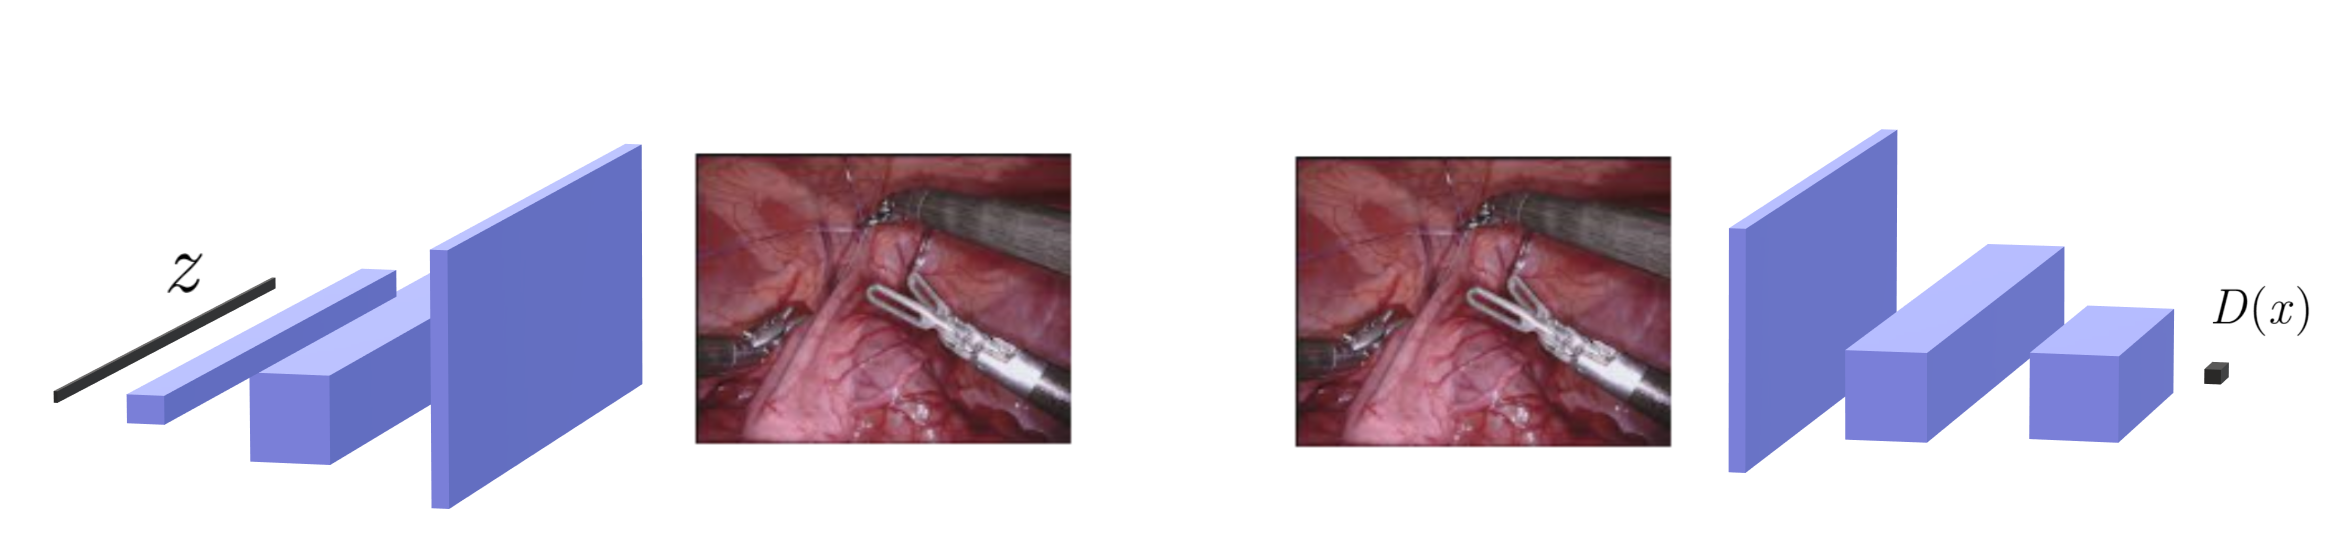
\includegraphics[width=15cm]{./images/gan_conv_image.png}
    \caption[GAN image generation.]{{On the left, an exemplary change in the dimensions of the feature maps in the generator is shown until an image is generated from the sample vector $z$.
        The right side refers to the calculation steps in the discriminator, where the probability $D(x)$, of which distribution the image comes from, is calculated.}\label{gan_conv_image}}
    \end{center}
\end{figure}
The purpose of the generator is to predict an output, that fits the distribution $p_{\text{data}}(x)$ of the training data $x$, through a generator function $G$.
The structure of this process corresponds to the following.
At first, a prior distribution $p_z(z)$ is defined, which is a random distribution to introduce randomness in the model. 
From this, a vector $z$ will be sampled and used as input to the generator function $G(z, \theta^g)$.
$\theta^g$ are the learnable weights of the generator network \cite{Goodfellow2020}.
In image-generation the generator model usually is a \acs{cnn} as described in section \ref{convnetworksection}.
The input vector $z$ will be passed to $G(z, \theta^g)$, where convolution layers will map its input to new feature maps using a suitable kernel dimension.
In this process, the dimensions of the feature maps of the respective layers are modified to finally match the output dimensions of an image.
The changes in the dimensions of the feature maps are shown in Figure \ref{gan_conv_image} exemplarily.
So the random vector $z$ will be processed by $G(z, \theta^g)$ to generate an artificial image as output $G(z)$.\\
%selbst ausgedacht vlt in ... \cite{Aggarwal2021} oder eher hier: Generative Adversarial Networks: An Overview

The task of the discriminator is to decide if a given input $x$ corresponds to the distribution of the training data or to the distribution of the generator.
In the case of image-generation, it determines whether $x$ is an image from the training data or an artificially generated image.
For this, a sample $x$ is passed through the network of the discriminator, which owns the weights $\theta^d$ \cite{Goodfellow2020}.
Therefore the discriminator function $D(x, \theta^d)$ returns a probability $D(x)$, that $x$ derives from the original training data instead of the generated distribution \cite{Goodfellow2014}.\\
In contrast to the generator the input to the discriminator, in this case an image, is downsized while it is processed through the network, as can be seen in Figure \ref{gan_conv_image}.
In the end the output $D(x)$ is often just a single value, which determines the probability.
% deconvolutional

\subsection{Adversarial training}\label{adversariallearning}
\begin{figure}[b]
    \begin{center}
     \includegraphics[width=15cm]{./images/Gan_struktur_cropped.pdf}
    \caption[GAN structure.]{{Schematic overview of how the training of a GAN is structured. The green line thereby represents the weight adjustment depending on $D(x)$.}\label{gan_schematic_fig}}
    \end{center}
\end{figure}
When it comes to the training of a GAN, both the weights of the discriminator and the generator have to be optimized.
Therefore the discriminator is trained to maximize the likelihood of correctly identifying both training data and samples from the artificial data $G(z)$.
The generator on the other hand learns from the results of the discriminator. 
This is done by minimizing $\log(1 - D(G(z)))$. 
In other words, the generator tries to fool the discriminator into making the prediction that a generated image $G(z)$ is an image from the training data.
% minimizing log(1−D(G(z))) is equivalent to minimizing (1−D(G(z)))
The minimum loss for the generator is reached when $D(x)$ will return a probability of one, that its input $G(z)$ is from the original distribution.
This means that the generator is able to successfully fool the discriminator \cite{Goodfellow2014}.
A schematic representation of the training is shown in Figure \ref{gan_schematic_fig}.\\
%Es wird davon ausgegangen, dass D einen a single scalar outputed.
The whole objective function $V(D,G)$ of a GAN can be written as shown in equation \ref{gan_equation}, taken from \cite{Goodfellow2014}:
\begin{equation}
    \min_{G}\max_{D}V(D,G) = \mathbb{E}_{x\sim p_{\text{data}}(x)}[\log D(x)]+\mathbb{E}_{z\sim p_z(z)}[\log(1-D(G(z)))]
    \label{gan_equation}
\end{equation}
The first term in the function $V(G,D)$ represents the expectation $E$ of the logarithm of the discriminator`s output, which stems from samplings $x$ of the training data $p_{\text{data}}(x)$.
In other words, the log-likelihood that the discriminator assigns the real sample $x$ to being an original sample.
The expectation hereby stands for calculating the average value of its operand for all samples of $x$.
This term is responsible for training the discriminator to identify real samples.
The second summand is the expected value of one minus the logarithm of the discriminator`s output $D(x)$ on generated data samples $G(z)$, which is the likelihood that the discriminator assigns the generator's output $G(z)$ to being a fake sample.
Hereby $z$ is a sample from the random distribution $p_z(z)$.\\
The function $V(D,G)$ can be seen as an adversarial loss because the generator $G$ and the discriminator $D$ should either minimize or maximize the value function $V(G,D)$ respectively.
This can be understood as playing a two-player min-max game against each other, where the networks have an opposing goal in the training process.\\
In the training of the basic GAN first, the weights of the generator are fixed and the discriminator is trained a previously defined number of times while maximizing the adversarial loss, so it makes better predictions of which distribution the sample comes from.
Then just the generator is trained and learns to adjust its generation output to correspond more to the distribution $p_{\text{data}}(x)$ of the training data through minimizing the objective function.
Therefore the discriminator performs worse because the generated samples are closer to the training distribution.
This process will be performed in an alternating way until the global optimum is found.
This is the case, when the distribution, that was learned from the generator, is equal to the real distribution $p_{\text{data}}(x)$ \cite{Goodfellow2014}.\\
In practice, this training process is not complex and most of the time an exact optimum cannot be found.
Instead, the models are trained until they converge and reach a stable equilibrium, where both models perform quite well.  
But also reaching this state can be compromised by different error sources.\\
Firstly the two networks can fail to converge, which means they don't reach a stable equilibrium of their losses.
So they can not play the min-max game effectively and do not reach the desired optimum.
If the hyperparameters are not set suitably, the generator, and discriminator won't balance themselves out and one of the networks will overpower the other.
That means that either the generator overfits the data and the discriminator can't learn to differentiate between the real and the fake input or the discriminator gets too good too fast and can't be fooled by the generator. 
Therefore the generator can not effectively learn how to generate an output that is close to the training distribution \cite{Creswell2018}.\\
Another problem is called mode collapse. 
This occurs when the generator learns a small set of outputs, that are all similar for different inputs.
But these results happen to be appropriate to trick the discriminator. Because of this, the GAN does not further adjust its generation process \cite{Creswell2018}.
If such a failure mode can be witnessed, an adjustment of the hyperparameters or a change in the structure of the network is necessary.

\section{Gan variants}\label{gan_var_l}
In this chapter, the the I2I translation networks CycleGAN and StarGAN are presented. 
Both networks will be described in detail, outlining their key characteristics and properties.
\subsection{Cycle GAN}\label{cyclegan}
The translation of images from the not smoked domain to the heavy smoked domain could help the segmentation network make more accurate predictions.
Therefore an image to image translation network can help in this task.
The goal of image translation is to learn the mapping of one image domain to another.
This is usually done using aligned image pairs.
An aligned image pair, for example, would be an image from the exact same position at day and at night.
But this kind of paired data is hard to acquire.
In the case of mapping medical images from a no smoke to a heavy smoke domain, it is not feasible to have the same images available with every instrument and organ in the same place while having smoke present in one and not the other.
Therefore an image translation without the need for aligned image pairs should be used.\\
It is also necessary that specific features that are not related to the smoke stay the same because the labeled segmentation masks should be used for training the segmentation network paired with the generated images.
Otherwise, a network, that is trained on the generated data, would learn false information if for example the appearance of surgical instruments is altered during the translation process.
An image to image translation model that can perform such a task is the CycleGan architecture proposed by Zhu et al. \cite{Zhu2017}.\\
The data here is also used in pairs, but each of them just has to belong to one of the domains, of which the mapping should be learned.
The idea is to use two generators and two discriminators, one for each domain.\\
The generator works in a similar way as in the traditional GAN structure, but it does not sample a random vector for generation.
Instead, it uses an encoder-decoder-like structure to first extract features from an image that should be translated into another domain.
This is done with three convolutional layers.
The first one has a kernel size of 7$\times$7 and stride one, to capture larger features from the image, followed by a convolution with a 3$\times$3 kernel and a stride of two.
Thereby the spatial dimensions of the input feature maps are reduced while the number of feature maps is increased.
The number of filters used from the first to the last convolution layers are: 64, 128, 256.
This way the generator can learn a more abstract representation of the features.\\
After each of those layers instance normalization and a ReLU activation function is used.
Instance normalization calculates the mean and variance for each input in the batch and normalizes them based on these values.
This may improve the performance of image-generation networks \cite{Ulyanov2016}.
The ReLU serves the purpose of introducing sparsity by zeroing all values below zero and therefore avoiding saturation in the network \cite{Sharma2020}.\\
Due to the choice of the number of filters the downsampling results in 256 feature maps, which are then passed to the residual blocks.
As the image size exceeds $256\times256$, nine of them are used, as stated in \cite{Zhu2017}.
These residual blocks contain two 3$\times$3 convolution operations are also followed by ReLU and instance normalization.
The purpose of the residual blocks is to learn the mapping of the feature maps from one domain to the other.\\
After processing through these residual layers, the features are upsampled with the transposed convolution operations corresponding to the two downsampling operations.\\
Then a last convolution operation with kernel size 7$\times$7 and a stride of one is used to generate an output with the same dimension as the input image.
Tangens hyperbolicus (tanh) is used to map the values in the output to the range of [-1, 1], so that it can be scaled to the range of pixel values [0, 255] without outliers.
The change in the feature dimensions of the individual steps in the generator can be seen in Figure \ref{cycle_gen_fig}.
\begin{figure}[bt]
    \begin{center}
     \includegraphics[width=15cm]{./images/gen_cycle.drawio.pdf}
    \caption[CycleGAN generator.]{{Visualization of the modifications regarding the feature maps in the generator.
    The green blocks indicate convolution operations, the red one represent residual blocks, and transposed convolution operations are visualized as blue blocks.
    The dimensions of the output are equal to those of the input image.
    Also, the changes in the height and width of the features depending on the size n of the input image are shown.
    }\label{cycle_gen_fig}}
    \end{center}
\end{figure}
The goal of the discriminator is to distinguish between generated images and those originating from the original dataset.
But instead of downsampling the input images to one value, here a PatchGAN architecture is used, as described in \cite{Isola2016}.
Hence the discriminator returns a two-dimensional matrix with a prediction in each entry.
The entries correspond to a certain area of the image and therefore the discriminator makes a prediction for each area of the image.\\
This is done by applying four 4$\times$4 convolution-InstanceNorm-LeakyReLU blocks, with the stride of the convolutions being two.
The number of filters used is from the first to the last convolution: 64, 128, 256, 512.
LeakyReLU is a variation of ReLU but instead of mapping negative values to 0, it multiplies them with a small constant, to allow non-zero gradients for backpropagation \cite{Sharma2020}.
Instance normalization is skipped for the first layer and the output of the area patches is calculated using a convolution, which combines the 512 feature maps into one output dimension.
The resulting values of the output are mapped to a value range between zero and one through a sigmoid function, indicating if the individual patches are from the generator (close to zero) or from the original data (close to one).\\
The described structure will produce an two-dimensional matrix with the output dimensions $\text{height}_{\text{input}}/2^4 \times \text{width}_{\text{input}}/2^4$, due to four convolutions with stride two.
Each entry thereby represents the discriminator's predictions for the corresponding area in the image.
It is to be noted, that the number of patches is determined through the convolution layers.
The more patches the more accurate the discriminator is but also more resource intensive.
As shown in \cite{isola2017image} a good tradeoff is achieved around a number of 70$\times$70 patches.
The process of how the discriminator calculates a prediction for an input image is shown in Figure \ref{cycle_disc_fig}.
Also, it ought to be remarked that a reflection padding of one is used in the first convolution of the generator and the discriminator, which means mirroring the border pixels of the images to mitigate errors in the edges of the image.\\
\begin{figure}[bt]
    \begin{center}
     \includegraphics[width=10cm]{./images/discriminator.drawio.pdf}
    \caption[CycleGAN discriminator.]{{Visualization of the modifications regarding the feature maps in the discriminator.
        The last convolution transforms the feature maps into the predictions for the corresponding areas in the image.
        Also, the changes in the height and width of the features depending on the size n of the input image are shown.
    }\label{cycle_disc_fig}}
    \end{center}
\end{figure}
To make the four networks work together following training structure is used, as proposed by Zhu et al. \cite{Zhu2017}.\\
There are two of the described generators and discriminators, one for each domain.
A generator $G_A$ is responsible for mapping images from domain $B$ to domain $A$ and one $G_B$ for the opposite case.
To train both of them to produce an output for the desired domain the discriminator networks $D_A$ and $D_B$ are used to create an adversarial loss like the one that is used in the objective function described in \ref{adversariallearning}:
\begin{equation}
    \mathcal{L}_{\text{adv}}(G_B, D_B, A, B) = \mathbb{E}_{b\sim p_{\text{data}}(b)}[\log D_B(b)]+\mathbb{E}_{a\sim p_{\text{data}}(a)}[\log(1-D_B(G_B(a)))]
    \label{adv_loss_cycle}
\end{equation}
This loss is further denoted as $\mathcal{L}_{\text{adv}}(G_B,D_B,A,B)$ for the adversarial loss of the generator $G_B$ and the discriminator $D_B$ for translating images from domain $A$ to $B$.
$\mathcal{L}_{\text{adv}}(G_A,D_A,B,A)$ would be the denotation for the other neural networks in the translation form $B$ to $A$.\\
It is also necessary that features that are not related to the specific domains remain the same in the translation process.
This is ensured by the cycle consistency loss.
The idea behind the cycle consistency loss is that if the generators $G_{A}$ and $G_{B}$ successfully learn the translation between the two domains, then applying for example $G_B$ to an image of $A$ to generate an artificial image of domain $B$ and then applying the other generator $G_A$ to it, it should result in a reconstructed image of domain $A$.
This reconstructed image should be close to the original input from $A$.
The Cycle consistency loss ensures consistent image-generation in CycleGAN by preserving the relevant information from the original input images.
It is defined as follows:
\begin{equation}
    \mathcal{L}_{\text{cyc}}(G_A, G_B) = \mathbb{E}_{a\sim p_{\text{data}}(a)}[\Vert G_A(G_B(a)) - a\Vert_1] + \mathbb{E}_{b\sim p_{\text{data}}(b)}[\Vert G_B(G_A(b)) - b\Vert_1]
\end{equation}
Hereby $\Vert G_A(G_B(a)) - a\Vert_1$ denotes the L1 norm of the cycled reconstruction image $G_A(G_B(a))$ minus the original image $a$.
The L1 norm, also known as Manhatten distance, sums up the absolute values of its input, which in this case results in an absolute difference between the two images.
$\mathbb{E}_{a\sim p_{\text{\text{data}}}(a)}$ denotes the expected value of the L1 norm over the data distribution $p_{\text{data}}(a)$, which means calculating the average value of the L1 norm for all samples of $a$.
%evtl. Expectation formula
% evtl L1 norm formel
This goes for both generators, respectively.
The mentioned losses are then combined to the total objective of the CycleGAN:
\begin{equation}
    \mathcal{L}(G_A, G_B, D_A, D_B) = \mathcal{L}_{\text{adv}}(G_A,D_A,B,A) + \mathcal{L}_{\text{adv}}(G_B,D_B,A,B) + \lambda \mathcal{L}_{\text{cyc}}(G_A, G_B)
    \label{objective_cyclegan}
\end{equation}
The $\lambda$ is hereby a choosable parameter, that adjusts the influence of the cycle consistency loss.
Because it is trained in an adversarial way the following equation has to be solved to get optimal generators $G_A^\ast$ and $G_B^\ast$:
\begin{equation}
    G_A^\ast, G_B^\ast = \text{arg} \underset{G_A, G_B}{\min}\underset{D_A, D_B}{\max}\mathcal{L}(G_A, G_B, D_A, D_B)
\end{equation}
This means finding the configurations $arg$ of the generators which minimize the loss function $\mathcal{L}(G_A, G_B, D_A, D_B)$, while at the same time the configuration of the discriminators should maximize this loss.
As described in section \ref{adversariallearning} this results in a min-max game, where both of the network pairs are trained in an alternating way.
This process is done until the generator and discriminator models converge to a stable state and no longer improve significantly with further training.
A schematic interaction of the individual networks can be seen in Figure \ref{cycle_gan_fig}.\\
\begin{figure}[bt]
    \begin{center}
     \includegraphics[width=15cm]{./images/CycleGan.drawio.pdf}
    \caption[CycleGAN structure.]{{Here the interaction of the individual networks in a CycleGAN training can be seen. 
    For the cycle consistency loss an image from domain $A$ is fed into the generator $G_B$ to generate an artificial image of domain $B$.
    This is used as input for the generator $G_A$ to generate a reconstructed image, which is compared to the original input with the cycle consistency loss, indicated by the black arrows.
    This process is also done for the images from domain $B$, but is not shown in the figure for the sake of clarity.
    The black dotted line shows the generation of an artificial image of domain $B$ which is given to the discriminator $D_B$ with original input from domain $B$ for the adversarial loss.
    This process is also executed for domain $A$ shown with the yellow dotted line. 
    }\label{cycle_gan_fig}}
    \end{center}
\end{figure}
Further adjustments that are made for a more stable training are to change the negative log-likelihood objective in the adversarial loss to a least-squares loss\cite{Zhu2017}.
Hereby the least squares loss can be understood as minimizing the mean squared error (MSE) error of the prediction.
\begin{equation}
    \text{MSE} = \frac{1}{n} \sum_{i=1}^{n} (y_i - \hat{y}_i)^2
\end{equation}
To implement this with a PatchGAN architecture the flattened output patches of the discriminator for a generated image $G_B(a)$ can be compared to a vector of the same length with ones in the case of training the generator.
This is because the training of the generator aims to make the discriminator falsely predict one for a generated image $G_B(a)$.
So the resulting value of the comparison of the prediction of a generated image and the vector with ones is to be minimized to maximize the adversarial loss.
For this comparison, the MSE is used.
Here $y_i$ is the vector with ones, $\hat{y}_i$ is the predicted patch value, and $n$ is the number of patches. 
It calculates the average squared difference between the vector and the predicted values.\\
In the case of training the discriminator the output of itself for a generated image should be zero, therefore the vector with ones is changed to a vector with zeros.
For an image of the original data one should be predicted and therefore the vector can remain being filled with ones before the mean square error is applied.
This way the MSE can be minimized during the whole training, while the comparison vector decides if the adversarial loss is minimized or maximized.\\
Also, there is the option to introduce yet another loss, called identity loss \cite{Zhu2017}.
The idea is to make the generator generate nearly the same image as the input if it is provided already in the target domain.
This loss can be defined as:
\begin{equation}
    \mathcal{L}_{\text{identity}}(G_A, G_B) = \mathbb{E}_{a\sim p_{\text{data}}(a)}[\Vert G_A(a) - a\Vert_1] + \mathbb{E}_{b\sim p_{\text{data}}(b)}[\Vert G_B(b) - b\Vert_1]
\end{equation}
Here the mean absolute difference between the output of the generator $G_A(a)$ that maps to domain $A$ and its input $a$ is calculated with the L1 norm $\Vert \cdot \Vert_1$.
The expectation of this term is calculated and summed up with the output of the same procedure for domain $B$, which will ensure an identity mapping if the input is already in the desired domain.
This loss is multiplied with a choosable parameter to determine its influence in the general loss and added to the total objective in formula \ref{objective_cyclegan}.

An additional adjustment is the use of a buffer to mitigate model oscillation.
This strategy proposed by Shrivastava et al. \cite{Shrivastava2016} involves updating the discriminators using a buffer of previously generated images instead of the ones generated directly before. 


\subsection{StarGAN}\label{star_gan}
StarGan is also an image-to-image translation model based on the GAN architecture proposed by Choi et al.\cite{choi2018stargan}.
It can perform multi-domain translation with a single generator, meaning it can not only translate images from one domain to another, but to multiple domains.
Additionally, the domains, also referenced as styles, can be combined to generate an output, that has the characteristics of different domains.
The main idea is to train the single generator with so-called domain label conditioning. %Zitat
Hereby information about the target domain is given to the generator in the translation process.\\
The following structure of the StarGAN is proposed by Choi et al.\cite{choi2018stargan}.
The structure of the generator in StarGAN is identical to the one used in CycleGAN.
The difference lies in the fact, that the input image of the generator is concatenated with a domain matrix, which serves as information about the domain the image should be translated to.
So assuming there are $n$ possible target domains, $n$ more layers of the dimensions $\text{height}_{\text{image}} \times \text{width}_{\text{image}}$ are attached to the image.
Each of these layers is either completely filled with ones or zeros, depending which domain serves as target for the translation.
So the first layer that is concatenated with the input represents the first domain, the second the second domain, and so on.
\begin{figure}[b]
    \begin{center}
     \includegraphics[width=5cm]{./images/Star_gan_gen_input.drawio.pdf}
    \caption[Domain concatenation StarGAN]{{Here the concatenation of the domain matrix with the input image can be seen. The result is the input for the generator.
    }\label{star_gan_input}}
    \end{center}
\end{figure}
This concatenation is shown in Figure \ref{star_gan_input}.
The concatenated input is given to the generator, which produces an image just like in the CycleGAN architecture.
This way the generator gets the information, to which domain he should translate the input image.
It is to be noted, that the domain matrix is not one hot encoded, so more than one layer can include ones to translate an image to different domains at once.
Also when dealing with translation with multiple domains this domain label conditioning allows the usage of only one generator.
Whereas otherwise, a separate generator would be necessary like in the CycleGAN, where for the translation between two domains two generators are used.\\
The discriminator is also based on a PatchGAN, but with a slightly different structure.
This is because it not only has to predict the distribution of which the input is coming from but also has to predict the source domain of its input.
It is structured as follows.
The input layer of the discriminator is a 4$\times$4 convolution with stride two, 64 filters, and a padding of one followed by a LeakyReLU.
In the hidden layer, there are five more convolutions of the same structure, but with a filter dimension that grows by two with each layer, which results in the following number of filters in this order: 128, 256, 512, 1024, 2048.
Each of those is also followed by a LeakyReLU.
The output layer is divided into two parts.
Firstly as in the CycleGAN, the outputs of the hidden layer are convoluted with a 3$\times$3 kernel, stride of one, and padding one.
This will generate prediction patches, that indicate the authenticity of an area in the input image.
The prediction of the discriminator regarding the origin of the input image is denoted as $D_{\text{src}}$.\\
Secondly, a convolution with $n$ filters for each domain in the specific case is applied to the output of the hidden layer.
The kernel size of this convolution is calculated as $\text{height}_{\text{image}}/2^k \times \text{width}_{\text{image}}/2^k$, whereby $k$ denotes the number of downsampling convolution operations performed beforehand.
In the explained case this would be six resulting from the input and hidden layer.
This output is a vector of length $n$, whereby each entry represents a prediction for the corresponding domains that are present in the input image.
The order of its entries is the same as for layers of the domain matrix concatenation in the generator.
This prediction is further denoted as $D_{\text{dom}}$.\\
To train the StarGAN, different loss functions are needed as proposed by Choi et al. \cite{choi2018stargan}.
To ensure a realistic generation of the images an adversarial loss is used.
Therefore the adversarial loss in the StarGAN for a sample distribution $p_{\text{data}}(x)$ is:
\begin{equation}
    \mathcal{L}_{\text{adv}} = \mathbb{E}_{x\sim p_{\text{data}}(x)}[\log D_{\text{src}}(x)]+\mathbb{E}_{x\sim p_{\text{data}}(x), d}[\log(1-D_{\text{src}}(G(x, d)))]
    \label{adv_loss_star}
\end{equation}
It works the same way as described in section \ref{adversariallearning}, where the goal of the generator $G$ is to minimize this loss whereas the discriminator $D$ tries to maximize it. 
The only difference is that the generator is conditioned on the target domain $d$ and also the expectation $\mathbb{E}_{x\sim p_{\text{data}}(x), d}$ is calculated for the samples $x$ with respect to the chosen target domain $d$.
However, because there is only one generator and discriminator the correct prediction and translation of the image domain is also to be learned.
For training the discriminator to identify the correct domain, the true domain class loss $\mathcal{L}_{\text{dom}}^t$ is defined as:
\begin{equation}
    \mathcal{L}_{\text{dom}}^t = \mathbb{E}_{x\sim p_{\text{data}}(x), d^\prime}[-\log D_{\text{dom}}(d^\prime|x)]
    \label{loss_dom_true}
\end{equation}
This true domain class loss calculates the expectation of the negative log probability of the original domain $d^\prime$ being predicted by the discriminator for an input image $x$.
Therefore when minimizing this loss the probability of the correct prediction of the true domain will rise.\\
Additionally, the generator should learn to translate an image $x$ to the domain $d$, on which it is conditioned to.
The probability of how correctly the generator has mapped the image to the right domain is decided through the discriminator, which makes a prediction of the domain of the image. 
This is ensured through the conditioned domain class loss:
\begin{equation}
    \mathcal{L}_{\text{dom}}^f = \mathbb{E}_{x\sim p_{\text{data}}(x),d}[-\log D_{\text{dom}}(d|G(x,d)]
    \label{loss_dom_false}
\end{equation}
Here the negative log probability of the conditioned domain $d$ being predicted by the discriminator for a generated image $G(x,d)$, which is conditioned with $d$, is calculated.
Of this probability, the expectation is formed over the samples from $p_{\text{data}}(x)$ with respect to the target domain $d$.
This way the generator is made to generate images in a domain, which is predicted correctly by the discriminator.\\
Furthermore a reconstruction loss is used, which should help to preserve the content in the image translation process that is not related to the target domain.
This is similar to the cycle consistency loss in the CycleGAN, but has to be implemented differently because there is only one generator. 
For this, an image $x$ is first translated to a target domain $d$ with the generator.
The output of this is again fed into the generator but conditioned to the original domain $d^\prime$ of the image, which should result in a reconstruction of the original image.
The values of the reconstruction image are subtracted from the values of the original image and from this in turn the L1 norm is calculated, which results in the absolute difference between the images.
If this difference is minimized, the reconstruction image is closer to the original, and therefore the generator produces an image that has similar characteristics as the input.
It can be written as follows:
\begin{equation}
    \mathcal{L}_{\text{rec}} = \mathbb{E}_{x\sim p_{\text{data}}(x),d,d^\prime}[\Vert x - G(G(x,d),d^\prime)\Vert_1]
    \label{loss_reconstruction}
\end{equation}
The presented loss functions are combined to the total objective of the discriminator $\mathcal{L}_D$ and for the generator $\mathcal{L}_G$:
\begin{equation}
    \mathcal{L}_D = -\mathcal{L}_{\text{adv}} + \lambda_{\text{dom}}\mathcal{L}_{\text{dom}}^t 
\end{equation}
\begin{equation}
    \mathcal{L}_G = \mathcal{L}_{\text{adv}} + \lambda_{\text{dom}}\mathcal{L}_{\text{dom}}^f + \lambda_{\text{rec}}\mathcal{L}_{\text{rec}}
\end{equation}
The adversarial loss $\mathcal{L}_{\text{adv}}$ is hereby negated for the discriminator, so if it is minimized the included losses are maximized.
The $\lambda$ parameters hereby are selectable to determine the influence of the individual losses.\\
During the training process, the target domain $d$ is chosen randomly, to ensure that all domains are covered.
\begin{figure}[bt]
    \begin{center}
     \includegraphics[width=10cm]{./images/star_gan.drawio.pdf}
    \caption[Training process StarGAN]{{Visualization of the training process of the StarGAN architecture.
    The original image is translated into a new domain. Then it is again translated to the original domain to create the reconstruction image, which is used for the reconstruction loss.
    Both the original and the translated image are used as input for the discriminator, which produces the probability of the origin $D_{\text{src}}$ to calculate the adversarial loss $\mathcal{L}_{\text{adv}}$.
    The discriminator also makes a prediction of the domain origin $D_{\text{dom}}$ of the translated and the original image, which is used for the true domain loss $\mathcal{L}_{\text{dom}}^t$ and the fake domain loss $\mathcal{L}_{\text{dom}}^f$.
    }\label{star_gan_training}}
    \end{center}
\end{figure}
The training process is visualized in Figure \ref{star_gan_training}.
To improve the training of the StarGAN, Choi et al. \cite{choi2018stargan} use an improved version of the adversarial loss of the Wasserstein GAN introduced by Gulrajani et al. \cite{Gulrajani2017}.
The idea of the original Wasserstein GAN as proposed by Arjovsky et al. \cite{Arjovsky2017} is to measure the distance between the real data and generated data for the adversarial loss.\\
The improved version of the adversarial loss used in StarGAN is an extension of the Wasserstein GAN's objective that enforces the Lipschitz continuity constraint using gradient penalty.
Enforcing the Lipschitz continuity constraint means that a function, in this case the discriminator, has to be Lipschitz continuous, which is defined for a function $f: \mathbb{R}^n \rightarrow \mathbb{R}^m$ on $X\subseteq\mathbb{R}^n$, as shown in equation \ref{lip_const}, taken from \cite{Fazlyab2019}:  
\begin{equation}\label{lip_const}
    \Vert f(x) - f(y) \Vert \leq L\Vert x - y \Vert \forall x,y \in X
\end{equation}
It states that the absolute difference between the function outputs $f(x)$ and $f(y)$ for any points in $X$ is not greater than a constant $L$ multiplied by the absolute difference between the input points $x$ and $y$ \cite{Fazlyab2019}.
Here $L$ is the Lipschitz constant, which denotes how fast the function can change while remaining Lipschitz continuous.
So enforcing the Lipschitz continuity constraint on the discriminator ensures that its output does not change too rapidly and thus helps stabilize the training process.
This is done by adding a gradient penalty to the adversarial loss, which is changed to the Wasserstein distance.
This results in an improved adversarial loss of: 
\begin{equation}
    \mathcal{L}_{\text{adv}} = \mathbb{E}_{x\sim p_{\text{data}}(x)}[D_{\text{src}}(x)]-\mathbb{E}_{x\sim p_{\text{data}}(x), d}[D_{\text{src}}(G(x, d)))] - \lambda_{\text{gp}}\mathbb{E}_{\hat{x}\sim p_{\text{data}}(\hat{x})}[(\Vert\nabla_{\hat{x}}D_{\text{src}}(\hat{x})\Vert_2 -1)^2]
    \label{impr_w_loss}
\end{equation} 
It is to be noted that when using this improved verion the discriminator should not have a sigmoid activation function to make a prediction of the image origin.
Instead, the raw values of the last convolution are used as a score, which is higher for real images and lower for generated images.
In the adversarial loss, seen in equation \ref{impr_w_loss}, the distance between the generated and original images is calculated as the difference of the scores of the original $D_{\text{src}}(x)$ and the generated images $D_{\text{src}}(G(x, d))$, by subtracting the expectations of the latter from the first.
To calculate the gradient penalty the interpolated point $\hat{x}$ is created through sampling between a real and a generated image.
The sampling is done in a straight line, which can be done using the following equation using a random number $\alpha \in [0, 1]$:
\begin{equation}
    \hat{x} = \alpha x + (1 - \alpha)G(x,d)
    \label{interpolated}
\end{equation}
Then the gradient $\nabla_{\hat{x}}D_{\text{src}}(\hat{x})$ of the discriminator with respect to the interpolated point $\hat{x}$ is calculated.
Finally, the gradient penalty is computed as the mean squared difference between the norm of gradients and one.
This gradient penalty is multiplied by a choosable lambda value $\lambda_{gp}$, which determines the influence on the adversarial loss.
The adversarial loss from equation \ref{adv_loss_star} is replaced by this loss.

%evtl. training with different datasets -> mask vector
%kein reflection padding
\section{Improving semantic segmentation}\label{seg_improve_gen}
\subsection{Augmenting data with artificial smoke images}
The initial situation is as follows: there are more frames in the no-smoke domain than in the heavy-smoke domain in all videos.
In order to improve the segmentation network, the ratio of no-smoke to heavy-smoke frames is adjusted during training.
First, the original ratio between the two domains is calculated. 
Then, this ratio is adjusted to create a predetermined ratio of the two domains, for example both domains should have an equal amout of images.
This is done by replacing the frames of the no-smoke domain with the same frames that have been translated into the heavy-smoke domain by an I2I translation network.
The images, which are replaced to obtain the predefined ratio, are chosen randomly each epoch.
With this setup, the segmentation network is trained in a usual way, but with an information gain for the heavy-smoke domain.
\subsection{GenSegNet}
\begin{figure}[b]
    \begin{center}
     \includegraphics[width=14cm]{./images/seg_gen_pdf.pdf}
    \caption[Training structure GenSegNet.]{{Adversarial training structure of the CycleGAN and the segmentation network in GenSegNet. The dotted lines represent the backpropagation to the individual networks.
    }\label{seg_gen_train}}
    \end{center}
\end{figure}
In this section, we propose a method to integrate the segmentation in the generation process and then use in turn the generation to improve the segmentation, called SegGenNet. 
Thereby the translation of images from the no-smoke domain to the heavy-smoke domain should be adjusted dynamically.
That means, while the segmentation network is trained, an image-to-image translation network should generate smoked images for the training.
At the same time, this translation network should be rewarded if it generates images, that are difficult to segment.
The idea is, that this way the artificially generated heavy-smoke images contain features like denser smoke or obscure the surgical instruments more because these are reasons for a more difficult segmentation.
This could in turn improve the segmentation as it receives new training data for particularly hard cases.\\
The image-to-image translation is done with a CycleGAN, because it focuses on the cycle consistency loss, which ensures the consistency and reversibility of the generation process.
This is important because the generated images must match the segmentation masks of the original image.
If the generation of hard-to-segment images is rewarded without cycle consistency, one possibility to reach this goal would be the creation of deformed instruments, which would not work for improving the segmentation.
As a segmentation network, the state of the art network DeepLabv3+ is used.\\
The training procedure is as follows.
For training the segmentation the Lovász loss $\mathcal{L}_{\text{lov}}(S(x), x^\prime)$ of the prediction $S(x)$ of the segmentation network and the ground truth $x^\prime$ should be minimized.
The CycleGAN on the other hand should maximize this loss for the generated images, while still retaining the goal of its original objective function described in equation \ref{objective_cyclegan}.
This leads to a new loss function of the CycleGAN of
\begin{equation}
    \begin{split}
    \mathcal{L}(G_A, G_B, D_A, D_B) = & \mathcal{L}_{\text{adv}}(G_A,D_A,B,A) + \mathcal{L}_{\text{adv}}(G_B,D_B,A,B) + \\
                                      &  \lambda_{\text{cyc}} \mathcal{L}_{\text{cyc}}(G_A, G_B) \\
                                      &  - \lambda_{\text{seg}}\mathcal{L}_{\text{lov}}(S(G(a)), a^\prime)
\end{split}
\label{objective_seg_gen_net}
\end{equation}
for a translation from the no-smoke domain $a$ to the heavy-smoke domain $b$.
Here the negated Lovász loss of the prediction of the segmentation network $S$ for a translated image $G_B(a)$ in the heavy-smoke domain and the ground truth $a^\prime$ is added to the original objective function. 
This way the generator $G_B$ for heavy-smoke-translation in the CycleGAN is rewarded if the segmentation network makes a poor prediction because then $\mathcal{L}_{\text{lov}}(S(G(a)), a^\prime)$ increases.
This loss is further referred to as segmentation reward.
It is to be noted that also the identity loss $\mathcal{L}_{\text{identity}}(G_A, G_B)$ like in the original CycleGAN can also be included.
The parameter $\lambda_{\text{seg}}$ denotes the influence of the segmentation reward on the image generation process.\\
When using this setup a pre-training of both models separately is necessary because the segmentation can only learn from realistic images and the generator needs a reasonably well segmentation prediction to be correctly rewarded.
The training procedure is as follows.
When training the segmentation network, each image is checked if it belongs to the heavy- or no-smoke domain and in that case is stored in an image buffer, that keeps the images of those domains in two separate lists.
Every $n$-th image is discarded from the image buffer to introduce randomness and to not degrade the segmentation network with too many images that may contain less information about the actual form of the surgical instruments.
The parameter $n$ can be freely chosen to adjust the training process.
If both lists in the buffer reach the chosen batch size of the segmentation network, the contained no-smoke images are translated by the CycleGAN into the heavy-smoke domain.
The translated images are first segmented by the DeepLabv3+ and the proposed loss of the CycleGAN from equation \ref{objective_seg_gen_net} is computed to train the CycleGAN.
Afterwards, the segmentation network is trained on those images instead of the actual images of the current batch.
It is to be noted, that the order of the dataset needs to be shuffled each epoch so that the same images are not always used for the image-to-image translation process.\\
This process represents an adversarial training where the training data of the segmentation network gets gradually harder to predict and the segmentation model learns to predict those hard-to-segment images.
The structure of this training can be seen in Figure \ref{seg_gen_train}.
% warum schlechter -> gleiche bilder hintereinander -> zu schwer zu segmentieren -> kann auch wieder nichts lernen



\chapter{Experiments and results}\label{result}
In this chapter, the evaluation criteria are presented first. 
Then, the experiments regarding I2I translation are depicted.
Subsequently, two experiments are conducted to explore the use of I2I techniques for improving segmentation.
\section{Evaluation Criteria}
In order to select which images are used for training the segmentation network, metrics should be used in addition to qualitative human evaluation.
Traditional evaluation metrics such as the accuracy and precision of the models are not fitting for evaluating GANs, as there is no ground truth to compare the generated data to.
Researchers have developed different approaches to overcome this challenge.
One of the most popular GAN evaluation metrics to evaluate the generated images is the Frechet Inception Distance (FID) \cite{alqahtani2019analysis}.
A different approach would be the Structural Similarity Index Measure (SSIM), which measures the image quality by comparing an original and a generated image. 
It was introduced by Wang et al. \cite{wang2004image}.
\paragraph{Fréchet inception distance}
The FID was introduced by Heusel et al. \cite{heusel2017gans} as a performance measure for GANs, which measures the similarity between two sets of images, in this case, the generated and the original images.
It is based on extracting high-level information from a generated and an original image by passing it through an Inception model.
The output features are then compared by the Fréchet distance.\\
The Inception model as proposed in \cite{szegedy2015going} is a deep CNN, which introduces inception modules.
These inception modules feature parallel convolution operations with different filter sizes to capture features at different scales, of which the results are concatenated and used as input for the next layer.
The inception blocks are then repeated to capture increasingly complex and abstract features.\\
To make the resulting vision-relevant features comparable, the mean and covariance over the set of the feature vectors of each image are calculated respectively.
It is assumed that the features follow a multidimensional Gaussian distribution with mean and covariance of the features \cite{heusel2017gans}.
The resulting distributions $F$ of an original and $G$ for a generated image are then compared using the Fréchet inception distance $d^2$ as defined in equation \ref{fid}, according to \cite{dowson1982frechet}:
\begin{equation}
    d^2(F,G) = |\mu_F - \mu_G|^2 + \text{Tr}(\Sigma_F + \Sigma_G - 2\sqrt{\Sigma_F \Sigma_G}),
    \label{fid}
\end{equation}
where $\text{Tr}$ denotes the trace operator, $\mu$ the mean, and $\Sigma$ the covariance matrix of the respective distribution.
The FID is typically calculated by computing the mean and covariance over a set of generated images and a set of original images separately and then using these values to measure the distance between the distributions using the Fréchet distance.
A lower FID score indicates that the two sets of images are more similar.

\paragraph*{SSIM}
The SSIM measure is based on the measurement of structural content $s$, luminance $l$, and contrast $c$. 
These values for an original image $x$ and a generated image $y$ can be compared as defined in equation \ref{ssim_l}, \ref{ssim_s}, and \ref{ssim_c}, according to~\cite{wang2004image}.
\begin{equation}
    l(x, y) =  \frac{2\mu_x\mu_y + C_1}{\mu^2_x + \mu^2_y + C_1}
    \label{ssim_l}
\end{equation}
\begin{equation}
    c(x, y) =  \frac{2\sigma_x\sigma_y + C_2}{\sigma^2_x + \sigma^2_y + C_2}
    \label{ssim_s}
\end{equation}
\begin{equation}
    s(x, y) =  \frac{2\sigma_{xy} + C_3}{\sigma_x\sigma_y + C_3}
    \label{ssim_c}
\end{equation}
Hereby, $\sigma$ denotes the standard deviation, $\mu$ the mean of the corresponding image, and the $C$ values a constant to improve numerical stability. 
The three measures are combined to the SSIM as defined in equation \ref{ssim_eq}, according to~\cite{wang2004image}.
\begin{equation}
    \text{SSIM}(x, y) = [l(x,y)]^\alpha \cdot [c(x,y)]^\beta \cdot [s(x,y)]^\gamma
    \label{ssim_eq}
\end{equation}
The parameters $\alpha$, $\beta$, and $\gamma$ regulate the influence of the individual measures. 
Hereby, a SSIM score of 1 means that the two images are identical regarding their structural information, while a score of 0 indicates no structural similarity at all.

\paragraph{Intersection Over Union and Dice Similarity Coefficient}
Two metrics that have proven to be effective for the segmentation of surgical tools are the Dice Similarity Coefficient and the Jaccard index \cite{leifman2022pixel}.
The Jaccard index as described in equation \ref{jaccard_index} is also known as the Intersection Over Union (IoU).
As a popular metric, it is used to evaluate the segmentation results.
For a pixel-wise prediction of the classes in an image, it can be implemented as adapted from \cite{leifman2022pixel}:
\begin{equation}
    \text{IoU}(A,B) = \frac{\sum_{i=1}^{|A|} a_i b_i}{\sum_{i=1}^{|A|} (a_i + b_i - a_i b_i)}
\end{equation}
for two binary segmentation masks $A$ and $B$ of the same size with the respective values $a$ and $b$ for each pixel position $i$.
Thereby, $a$ and $b$ have a value of 0 for background and 1 if the class for which the metric is calculated occurs there.
Another way of calculating this metric is with a confusion matrix, where all true positives (TP), false positives (FP), true negatives (TN), and false negatives (FN) are calculated for each prediction and ground truth of the segmentation masks.
The IoU for a class $c$ can be calculated as described in \cite{sulistiyo2018attribute}:
\begin{equation}
     \text{IoU}_c = \frac{\text{TP}_c}{\text{TP}_c + \text{FP}_c + \text{FN}_c}
\end{equation}
This is calculated for each class of surgical instruments that occur in the data of the current task.
To get the mean IoU (mIoU) for the whole data, the IoU values for each class are summed and then divided by the number of classes $C$:
\begin{equation}
    \text{mIoU} = \frac{1}{C}\sum_{i=1}^{C} \frac{\text{TP}_c}{\text{TP}_c + \text{FP}_c + \text{FN}_c}
\end{equation}
The IoU for the background is not included, because it is considered not a relevant class.\\
The Dice Similarity Coefficient also measures the overlap between the predicted segmentation mask and the ground truth mask.
It is calculated as twice the intersection of the predicted and ground truth masks divided by the sum of their areas.
The Dice Similarity Coefficient is defined as in \cite{leifman2022pixel}:
\begin{equation}
    D(A,B) = \frac{2|A \cap B|}{|A| + |B|}
\end{equation}
Thus, using true positives and false negatives, the Dice coefficient can be defined as follows:
\begin{equation}
    \text{Dice} = \frac{2\text{TP}}{2\text{TP} + \text{FP} + \text{FN}}
\end{equation}
Therefore, the mean Dice (mDice) can be calculated as:
\begin{equation}
    \text{mDice} = \frac{1}{C}\sum_{i=1}^{C} \frac{2\text{TP}_c}{2\text{TP}_c + \text{FP}_c + \text{FN}_c}
\end{equation}
Both, IoU and Dice range from zero to one with zero indicating no overlap between the predicted and ground truth masks, while a value of one represents complete overlap between the two masks.
% was sind gute scores für miou
% was sind gute scores für dice

\section{Image to image translation}\label{i2i_trans}
In this section the CycleGAN and StarGAN architecture are used to translate images into images with artificial smoke.
\subsection{CycleGAN}\label{cyclegan_experiment}
A CycleGAN with an architecture as described in section \ref{cyclegan} is used to translate images from the no-smoke domain to the heavy-smoke domain.
Also, the identity loss was used for training the CycleGAN, because it seems to help preserve the overall structure of the image. 
Adam is used to optimize the generators and discriminators to speed up the convergence of both networks and improves the overall performance of the CycleGAN.
Hereby the beta values are set to 0.5 for $\beta_1$ and 0.999 for $\beta_2$.\\
An image buffer, which holds up to 20 images is implemented to reduce the oscillation in the training process.
A one-cycle scheduler as proposed in \cite{smith2018disciplined} is used for adjusting the learning rate during training for faster convergence of the network.
The learning rate starts hereby at a lower value, increases to the maximum set value in the middle of the training process, and then decreases again towards the end of the training, shown exemplarily in Figure \ref{one_cycle}.
For implementation, the Pytorch OneCycleLR is used with a percentage start (pct) of 0.05 meaning the learning rate will increase for the first five percent of the total amount of steps and afterward starts decreasing.
An example of the adjustment of the learning rate is given in Figure \ref{one_cycle}.
\begin{figure}[tb]
    \begin{center}
     \includegraphics[width=8cm]{./images/once_cycle.pdf}
    \caption[One-cycle scheduler]{{Exemplary learning rate adjustment with one-cycle scheduler for 86,190 steps and pct start of 0.05.
    }\label{one_cycle}}
    \end{center}
\end{figure}
\paragraph*{Data} 
The generated images should be in the heavy-smoke domain because it is assumed that this will have the greatest benefit in training the segmentation.
The images which are translated are from the no-smoke domain as these are the most present.
Therefore the training data consists of images from the no- and heavy-smoke domains.
The dataset for training returns a batch of random pairs of these domains.
Because of the tanh activation function used in this model, the image values have to be in the same range of [-1,1] as tanh.
This is done by dividing the pixel values by the maximal pixel value of 255.
Then they are normalized with a mean and standard deviation of 0.5.
Therefore the generated images are in the same value range as the original ones.
Otherwise, the discriminator could detect the original images based on value outliers.\\
Due to computational limitations, the images are downsized by a factor of two.
The original images are in a resolution of $1920\times1080$ pixels, so they are downsized to $960\times540$.
Because for the validation of the segmentation network a six-fold cross-validation is used, the same folds should be used for training the CycleGAN to not introduce information about the validation data.
The training data for each fold contains the images of five out of the six videos.
In the following, training fold one means omitting video one, and therefore videos two to six are used for training. 
\paragraph{Hyperparameters} The hyperparameters for the model are chosen as follows.
A batch size of two is used due to memory limitations.
To initialize the model, all of the weights were set to values from a Gaussian distribution $N(0, 0.02)$, which has been found to be a suitable starting point for this particular architecture \cite{Zhu2017}.
The learning rate of the generator and discriminator is set to $10^{-4}$, which is the highest learning rate, where the networks converge to a stable equilibrium. 
Adopted from the original CycleGAN the lambda values for the cycle-consistency loss are set to ten and the lambda for the identity loss to five.\\
\paragraph*{Training}
\begin{figure}[bt]
    \centering
    \subfloat[Loss of discriminator for no-smoke images.]{\includegraphics[width=0.49\textwidth]{./images/plots_cyclegan/disc_ns_loss.pdf}\label{fig:disc_ns_loss}}
    \hfill
    \subfloat[Loss of discriminator for heavy-smoke images.]{\includegraphics[width=0.49\textwidth]{./images/plots_cyclegan/disc_hs_loss.pdf}\label{fig:disc_hs_loss}}
    
    \vspace{0.5cm}
    
    \subfloat[Loss of generator for no-smoke images.]{\includegraphics[width=0.49\textwidth]{./images/plots_cyclegan/gen_ns_loss.pdf}\label{fig:gen_ns_loss}}
    \hfill
    \subfloat[Loss of generator for heavy-smoke images.]{\includegraphics[width=0.49\textwidth]{./images/plots_cyclegan/gen_hs_loss.pdf}\label{fig:gen_hs_loss}}
    
    \caption[CycleGAN loss curves]{Display of the loss values for the domain-specific generator and discriminator during training.}\label{fig:cycle_disc_gen_loss}
\end{figure}
The model was trained for 30 epochs, as no further improvement of the generated data was observed afterward.
Figure \ref{fig:cycle_disc_gen_loss} displays the change in the discriminator and generator loss during training, with values averaged over one epoch, whereby in the individual steps, the oscillation is much higher.
The generators and discriminators converge around epoch seven.
The loss value for the discriminator saturates at around 0.4, which is a value that provides enough information for the generator to learn how to fool the discriminator, while still penalizing images that are too far from the original image distribution.\\
Due to its architecture, the CycleGAN produces artificial images of both domains, heavy-smoke and no-smoke.
The evaluation of these is focused on the heavy-smoke images only, because they are the only ones used to enhance the segmentation training.
To evaluate the generated images the FID is computed by comparing the Gaussian distributions of the generated heavy-smoke images with the distribution of original heavy-smoke images because the similarity of the images should be tested not only regarding the general structure but also regarding the occurrence of smoke.
Therefore, the mean and standard deviation of both the generated and original images are updated on a per-image basis, with an equal number of updates applied to each.
After updating the means and standard deviations of the generated and original images for one epoch, the FID between the resulting distributions is calculated.
The SSIM is calculated with one generated and one original heavy-smoke image at once, to set the focus of this metric more on the smoke generation like in the FID.
The resulting values are averaged over one epoch.
The progress of both metrics during training is shown in Figure \ref{fig:cycle_metrics}.
\begin{figure}[tb]
    \centering
    \subfloat[SSIM in CycleGAN training.]{\includegraphics[width=0.49\textwidth]{./images/plots_cyclegan/ssim_cycle.pdf}\label{fig:ssim_cycle}}
    \hfill
    \subfloat[FID in CycleGAN training.]{\includegraphics[width=0.49\textwidth]{./images/plots_cyclegan/fid_cycle.pdf}\label{fig:fid_cycle}}
    \caption[FID and SSIM of CycleGAN]{Display of the FID and SSIM values evaluated every 5 epochs.}\label{fig:cycle_metrics}
\end{figure}
The FID is decreasing for all folds until epoch 20, where it reaches its minimum. 
After that, a slight increase can be seen.
The SSIM grows for fold 5 until epoch 30, fold one and two saturate after epoch 25, and a slight decrease occurs after epoch 20 for fold 3, 4, and 6.
This indicates that the optimum is around epoch 20.
Human evaluation comes to a correlating result, by comparing random generated images in the different epochs as shown in Figure \ref{fig:cycle_img_train}.
\begin{figure}[tb]
    \centering
    \subfloat[Original image.]{\includegraphics[width=0.49\textwidth]{./images/CycleGAN_imgs/f_8550_artifact_org.png}\label{fig:art_o}}
    \hfill
    \subfloat[Generated image after 5 epochs.]{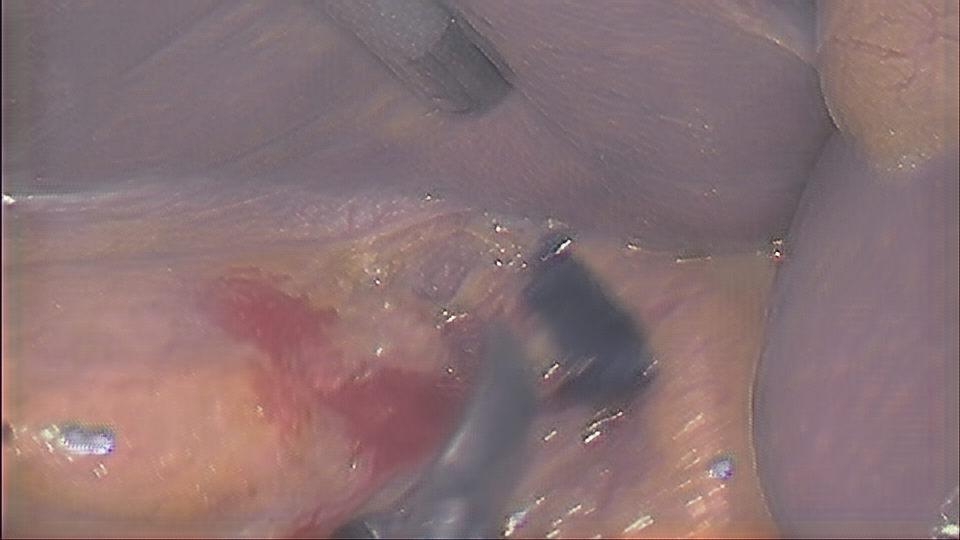
\includegraphics[width=0.49\textwidth]{./images/CycleGAN_imgs/f_8550_artifact_5.png}\label{fig:art_5}}
    
    \vspace{0.5cm}
    
    \subfloat[Generated image after 20 epochs.]{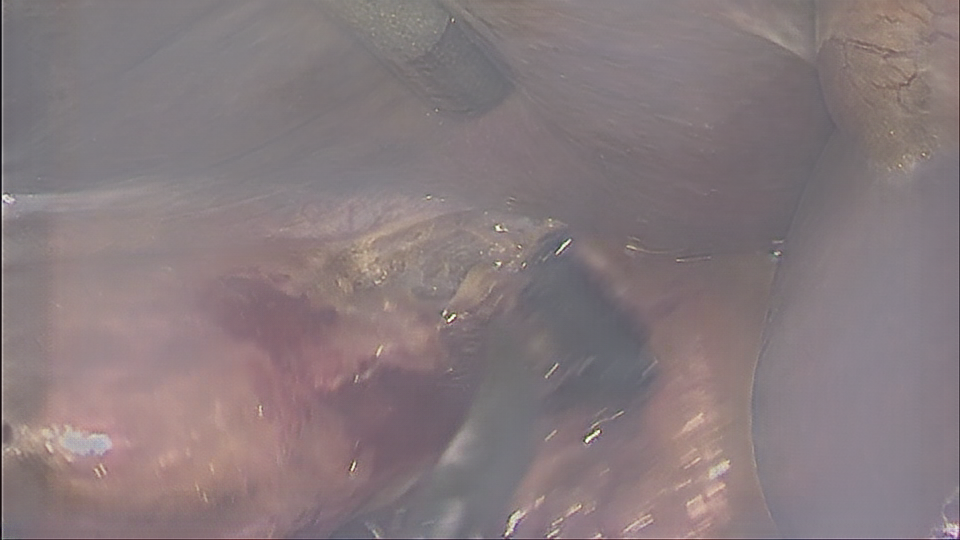
\includegraphics[width=0.49\textwidth]{./images/CycleGAN_imgs/f_8550_artifact_20.png}\label{fig:art_20}}
    \hfill
    \subfloat[Generated image after 30 epochs.]{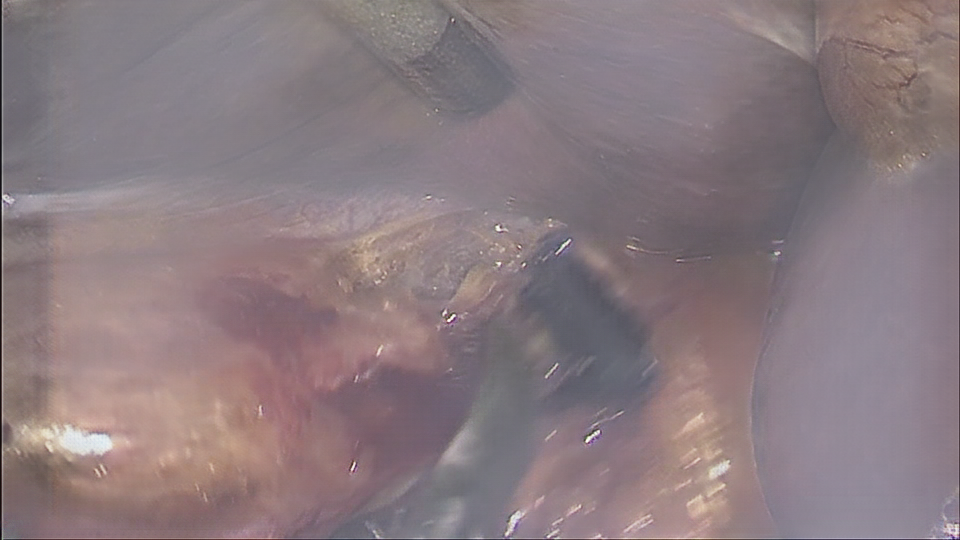
\includegraphics[width=0.49\textwidth]{./images/CycleGAN_imgs/f_8550_artifact_30.png}\label{fig:art_30}}
    \caption[Image generation of CycleGAN]{Image generation process at different epochs, taken from video 6 frame 8550 of fold 2.}\label{fig:cycle_img_train}
\end{figure}
In Figure \ref{fig:art_30} it can be seen, that artifacts like the dark bar on the left side of the image are more prominent than in the previous epochs.
On a different note, in epoch 5 of the generation process also a little artifact around the reflection in the left corner can be seen.
The generated image of epoch 20 seems like a good tradeoff. Additionally, the generated smoke seems a bit more dense than in the other steps.\\
Since metrics like SSIM or FID can also find correlations that are not immediately obvious to the human eye, the metrics should also be taken into account.
Therefore, the images, generated in epoch 20, have been selected as the most optimal representations based on the evaluation metrics and subjective human assessment.
Figure \ref{fig:cycle_showcase} presents a comparison of the generated images with their corresponding originals.
Table \ref{fid_ssim_cycle_table} presents the SSIM and FID values that indicate the best results.
\begin{table}[!tb]\vspace{1ex}\centering
    \caption[Metrics CycleGAN]{FID and SSIM values for evaluation at epoch 20.\label{fid_ssim_cycle_table}}
    \begin{tabular*}{8cm}{ll|@{\extracolsep\fill}cccc}
    &&\multicolumn{2}{c}{Metric} \\
    && FID & SSIM  \\\hline
    %\multirow{6}*{\rotatebox{90}{Domain}}
    & Fold 1 &  39.55  & 0.7860 \\%\cline{2-6}
    & Fold 2 & 44.21  &  0.7749 \\%\cline{2-6}
    & Fold 3 & 40.26  &  0.7891\\%\cline{2-6}
    & Fold 4 & 44.55  &  0.7914\\%\cline{2-6}
    & Fold 5 & 41.42  &  0.7818\\%\cline{2-6}
    & Fold 6 & 41.05 &  0.7844\\\hline
    & mean & 41,84 & 0.7846\\
    \end{tabular*}
    \captionsetup{justification=centering}
\vspace{2ex}\end{table}
\begin{figure}[bt]
    \centering
    \subfloat[Original HS.]{\includegraphics[width=0.25\textwidth]{./images/CycleGAN_imgs/showcase/f_17004_original_smoke.png}\label{fig:org_cycle_1}}
    \hfill
    \subfloat[Original HS.]{\includegraphics[width=0.25\textwidth]{./images/CycleGAN_imgs/showcase/f_18003_original_smoke.png}\label{fig:org_cycle_2}}
    \hfill
    \subfloat[Original HS.]{\includegraphics[width=0.25\textwidth]{./images/CycleGAN_imgs/showcase/f_26006_original_smoke.png}\label{fig:org_cycle_3}}
    \hfill
    \subfloat[Original HS.]{\includegraphics[width=0.25\textwidth]{./images/CycleGAN_imgs/showcase/f_28000_original_smoke.png}\label{fig:org_cycle_4}}
    \vspace{0.5cm}
    \subfloat[Original NS.]{\includegraphics[width=0.25\textwidth]{./images/CycleGAN_imgs/showcase/f_6600_org.png}\label{fig:cycle_org1}}
    \hfill
    \subfloat[Generated HS.]{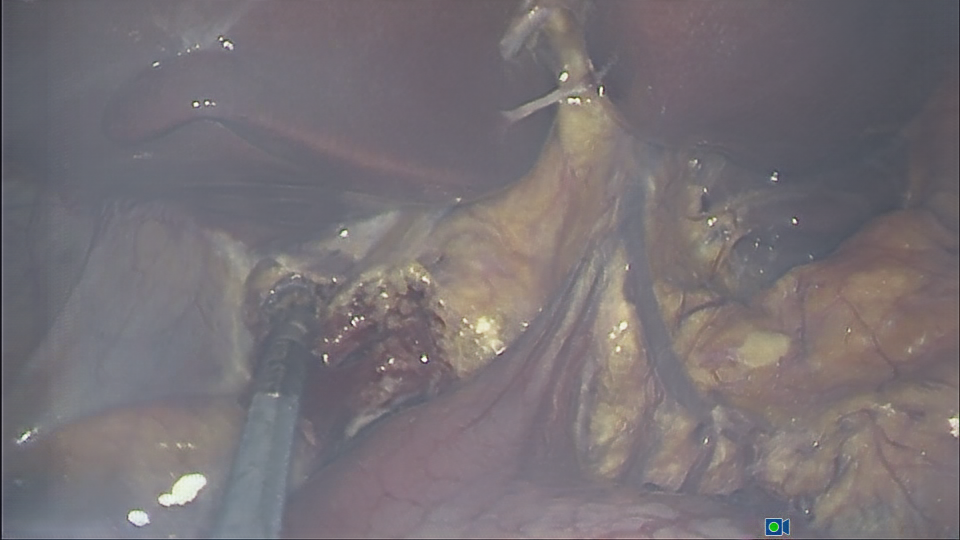
\includegraphics[width=0.25\textwidth]{./images/CycleGAN_imgs/showcase/f_6600.png}\label{fig:cycle_gen1}}
    \hfill
    \subfloat[Original NS.]{\includegraphics[width=0.25\textwidth]{./images/CycleGAN_imgs/showcase/f_7075_org.png}\label{fig:cycle_org2}}
    \hfill
    \subfloat[Generated HS.]{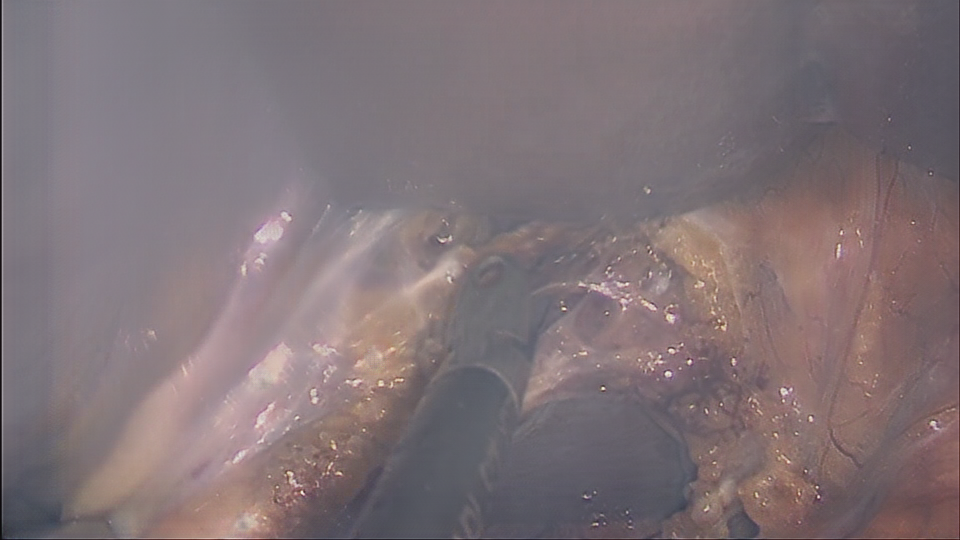
\includegraphics[width=0.25\textwidth]{./images/CycleGAN_imgs/showcase/f_7075.png}\label{fig:cycle_gen2}}
    \vspace{0.5cm}    
    \subfloat[Original NS.]{\includegraphics[width=0.25\textwidth]{./images/CycleGAN_imgs/showcase/f_12150_org.png}\label{fig:cycle_org3}}
    \hfill
    \subfloat[Generated HS.]{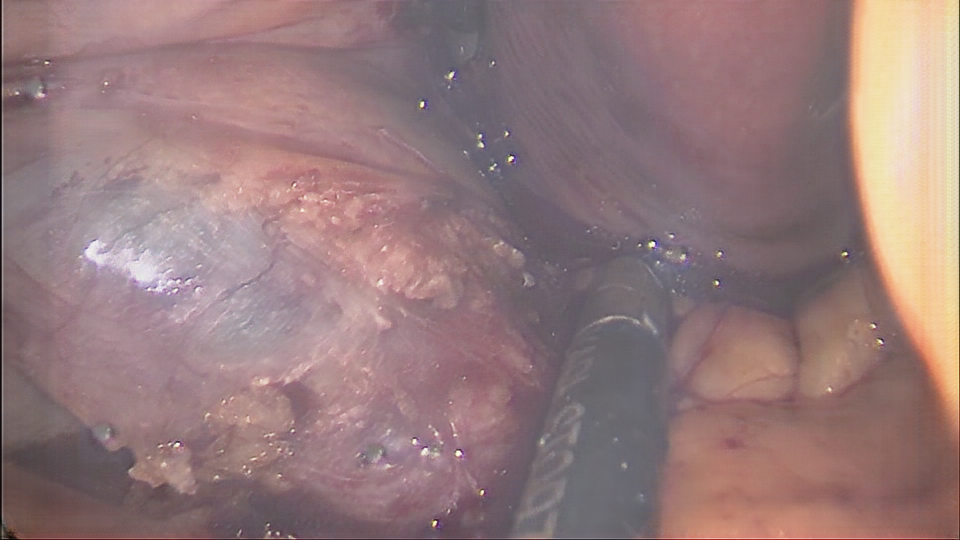
\includegraphics[width=0.25\textwidth]{./images/CycleGAN_imgs/showcase/f_12150.png}\label{fig:cycle_gen3}}
    \hfill
    \subfloat[Original NS.]{\includegraphics[width=0.25\textwidth]{./images/CycleGAN_imgs/showcase/f_12750_org.png}\label{fig:cycle_org4}}
    \hfill
    \subfloat[Generated HS.]{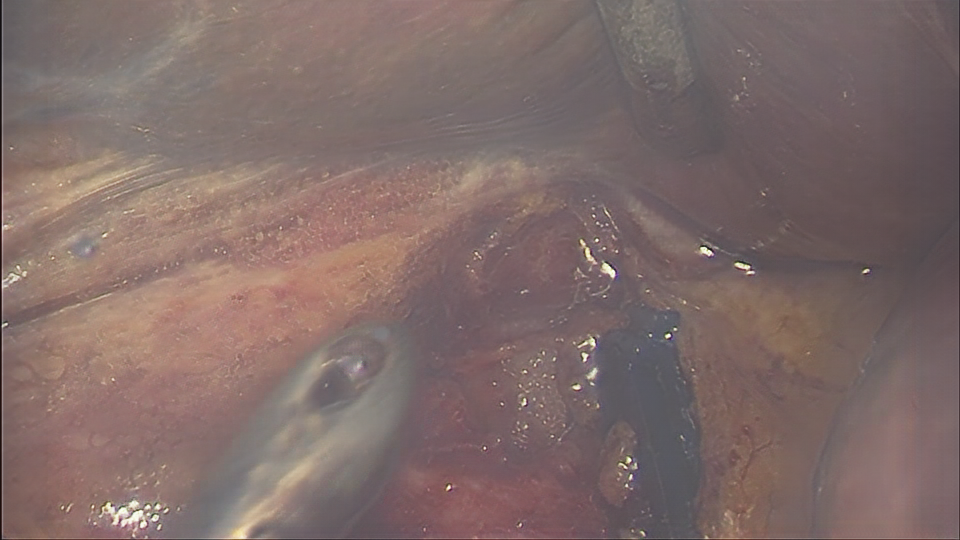
\includegraphics[width=0.25\textwidth]{./images/CycleGAN_imgs/showcase/f_12750.png}\label{fig:cycle_gen4}}
    \vspace{0.5cm}
    \caption[Generated images of CycleGAN.]{(a)-(d) representing original images in the heavy-smoke domain, (e),(g),(i),(k) original images from the no-smoke domain, and (f),(h),(j),(l) generated images from the corresponding original image shown in (e),(g),(i),(k).}\label{fig:cycle_showcase}
\end{figure}
\FloatBarrier
%-> FID und SSIM tabelle?
%-> oszillation nochmal in grafik darstellen
%-> schreiben was ist discriminator loss genau? 
%\clearpage
\subsection{StarGAN}
A StarGAN model is used to generate not only heavy-smoke images but also slight-smoke images due to its ability to translate into multiple domains.
For this, the architecture described in \ref{star_gan} is used.
To preserve the original structure of the image, an identity loss as in the CycleGAN is introduced in addition to the reconstruction loss.
This is done by conditioning the generator to translate an image to its original domain, which should result in the identity of the original image.
This identity is compared to the source image by calculating the mean absolute error and this loss is added to the general objective of the StarGAN.
The use of a one-cycle learning rate scheduler and the Adam optimizer proved to be effective in training the CycleGAN model, which is why they are also used here in the same configuration.\\
Due to its similar generator, the images to be translated are pre-processed in the same way as in the CycleGAN model.
For conditioning, the generator to translate an image to the desired domain, a one-hot encoded vector of length three is defined with position one denoting no smoke, two slight smoke, and three heavy smoke.
This vector is used to compare the results of the discriminators' class prediction to the ground truth and create the input condition matrix, which is concatenated with the input image.
The original images are loaded randomly as no pairing is required due to the conditioning.
\paragraph{Hyperparameters} The hyperparameters for the model are chosen as follows.
Because of its reduced model size a batch size of six is chosen.
The learning rate for the generator and discriminator is set to $2 \cdot 10^{-4}$.
To adjust the influence of the different loss functions, the lambda values used are 10 for the reconstruction loss, 1 for the domain classification loss, 4 for the identity loss, and 10 for the gradient penalty.
The weights of the model are initialized with values from a Gaussian distribution of $N(0, 0.02)$.
\paragraph{Training} The training consisted of optimizing the model parameters for 30 epochs, whereby the images are loaded in random order in a batch.
The target domain of each image is assigned randomly, whereby the source domain of the image won't be chosen.
Figure \ref{fig:star_train} shows the loss of the generator and discriminator.
\begin{figure}[tb]
    \centering
    \subfloat[Generator with reconstruction loss and classification loss]{\includegraphics[width=0.33\textwidth]{./images/plot_stargan/g_loss_star.pdf}\label{fig:g_star}}
    \hfill
    \subfloat[Generator loss only.]{\includegraphics[width=0.33\textwidth]{./images/plot_stargan/g_loss_oscill_star.pdf}\label{fig:g_star_oscil}}
    \hfill
    \subfloat[Generated class loss.]{\includegraphics[width=0.33\textwidth]{./images/plot_stargan/g_loss_class_star.pdf}\label{fig:g_star_class}}
    
    \vspace{0.5cm}
    
    \subfloat[Discriminator loss fake \\ images.]{\includegraphics[width=0.33\textwidth]{./images/plot_stargan/d_loss_fake_star.pdf}\label{fig:d_star_fake}}
    \hfill
    \subfloat[Discriminator loss original images.]{\includegraphics[width=0.33\textwidth]{./images/plot_stargan/d_loss_real_star.pdf}\label{fig:d_star_real}}
    \hfill
    \subfloat[Discriminator class loss.]{\includegraphics[width=0.33\textwidth]{./images/plot_stargan/d_loss_class_star.pdf}\label{fig:d_star_class}}
    \caption{Loss representations during the training of StarGAN.}\label{fig:star_train}
\end{figure}
Hereby the combined generator loss shown in Figure \ref{fig:g_star} includes the identity and reconstruction loss, which, when decreasing as in this case, indicates a working training.
The generator loss in Figure \ref{fig:g_star_oscil} is based on the prediction of the discriminator for generated images and is, therefore, the negated equivalent to the discriminator loss for generated images shown in Figure \ref{fig:d_star_fake}. 
The plotted curve appears to be oscillating with a slight negative offset, meaning it does not overpower the discriminator nor the other way around.
The discriminator makes more stable predictions for real images while oscillating stronger for generated images.
It is to be noted that the loss values of the discriminator are scores and not predictions like in the CycleGAN, due to the usage of the Wasserstein loss.
Also, it is to be seen, that the domain classification loss for both, the generator and discriminator, shown in Figure \ref{fig:d_star_class} and \ref{fig:g_star_class} are converging to zero.\\
To evaluate the images the FID is calculated in the same way as for the CycleGAN, described in section \ref{cyclegan_experiment}, but in addition to the heavy-smoke images also the mean and standard deviation of the slight-smoke images are added to the Gaussian distribution of generated and original images respectively.
After calculating the distributions the FID for the generated and original distributions is computed.
The SSIM also takes the slight-smoke images into account, meaning that the SSIM is calculated for every generated slight- and heavy-smoke image paired with an original in the corresponding domain.
The progress of both metrics during training is shown in Figure \ref{fig:star_metric_plots}.
\begin{figure}[tb]
    \centering
    \subfloat[FID during training.]{\includegraphics[width=0.45\textwidth]{./images/plot_stargan/fid_star.pdf}\label{fig:star_fid}}
    \hfill
    \subfloat[SSIM during training.]{\includegraphics[width=0.45\textwidth]{./images/plot_stargan/star_ssim.pdf}\label{fig:ssim_fid}}
    \caption{Representation of the metric values for generated images during the training of StarGAN.}\label{fig:star_metric_plots}
\end{figure}
The two metrics, FID and SSIM, do not have a clear optimum.
Both metrics show fluctuations, and there is no clear trend of improvement over the course of training. 
When considering human evaluation, it is clear that some images exhibit noticeable artifacts, particularly in the slight-smoke domain.
In general, the quality of the output is lower than that of CycleGAN, as evidenced by the lower values of both metrics in all folds and by visual inspection of the images.
Based on the images shown in Figure \ref{fig:star_showcase}, it can be observed that the smoke generation increases over the course of the training.
However, there are noticeable artifacts and imperfections in the generated slight-smoke images.
While the heavy-smoke images appear adequate, they do not match the quality of the generated images of the CycleGAN.
\begin{figure}[bt]
    \centering
    \subfloat[Generated HS in epoch 5.]{\includegraphics[width=0.33\textwidth]{./images/images_star/f_15075_v3_hs_ep5.png}\label{fig:starimghs1}}
    \hfill
    \subfloat[Generated HS in epoch 20.]{\includegraphics[width=0.33\textwidth]{./images/images_star/f_7450_hs_v4_ep20.png}\label{fig:starimghs2}}
    \hfill
    \subfloat[Generated HS in epoch 30.]{\includegraphics[width=0.33\textwidth]{./images/images_star/f_7450_hs_v2_ep30.png}\label{fig:starimghs3}}
    \vspace{0.5cm}
    \subfloat[Generated SS in epoch 5.]{\includegraphics[width=0.33\textwidth]{./images/images_star/f_6100_v3_ms_ep5.png}\label{fig:starimgms1}}
    \hfill
    \subfloat[Generated SS in epoch 20.]{\includegraphics[width=0.33\textwidth]{./images/images_star/f_7825_ms_v4_ep20.png}\label{fig:starimgms2}}
    \hfill
    \subfloat[Generated SS in epoch 30.]{\includegraphics[width=0.33\textwidth]{./images/images_star/f_10375_2_ms_ep30.png}\label{fig:starimgms3}}
     \vspace{0.5cm}
    \caption[Generated images StarGAN]{Display of the images generated heavy-smoke (HS) and slight-smoke (SS) during training the StarGAN at different epochs.}\label{fig:star_showcase}
\end{figure}

%\clearpage
\FloatBarrier
\section{Augmenting data with artificial smoke images}\label{experiment_enhance1}
The generated images are intended to be integrated into the segmentation process to improve its performance.
The baseline will be explained first to enable a comparison between the segmentation results obtained with the generated images and those obtained using the baseline segmentation.
\paragraph{Baseline configuration} The baseline configuration involves the use of a DeepLabv3+ for semantic segmentation.
The DeepLab architecture is constructed as described in section \ref{dlv3_section}.
The baseline approach was implemented using a batch size of 18 and a learning rate of 0.0001.
The Lovász loss function was employed as loss function, as it has been shown to be effective for semantic segmentation tasks.
To further improve training, the one-cycle scheduler was utilized to adjust the learning rate during the course of the training process with a percentage start of 0.05.
Finally, the Adam optimizer was selected with beta values of $0.9$ for $\beta_1$ and 0.999 for $\beta_2 $.
To achieve better results, the model parameters of DeepLabv3+ are loaded from a model pre-trained on the Cityscapes \cite{cordts2016cityscapes} dataset.
Furthermore, a resnet-101 as introduced in \cite{He2015} is used as backbone for the DeepLabV3+.\\
For training and validation, the images are resized to $912\times513$ for computational reasons.
In addition to resizing, the pixel values of the images are standardized, meaning they have a mean of zero and a standard deviation of one.
This can help prevent numerical instability during training and give equal importance to all features, which results in more accurate predictions.%quelle zu standardization
This is done by subtracting the mean value from each pixel and then dividing by the standard deviation. 
The mean and standard deviation are calculated from the pixel values of the used training dataset.
These values are shown in Table \ref{std_mean_table} for the images of the used videos.\\
\begin{table}[b]\vspace{1ex}
    \centering
    \caption[Mean and standard deviation]{Mean and standard deviation for each channel.\label{std_mean_table}}
    \begin{tabular*}{15cm}{l|@{\extracolsep\fill}cccc}
    &\multicolumn{3}{c}{Normalization values} \\
    & Red channel & Green channel & Blue channel  \\\hline
    %\multirow{2}*%{\rotatebox{90}{}}\multirow{6}*{\rotatebox{90}{Domain}}
    Mean & 0.51948161  & 0.38390668 & 0.35970329 \\%\cline{2-6}
    standard deviation & 0.18273795 &  0.15816768 &  0.15964756\\\hline
    \end{tabular*}
    \captionsetup{justification=centering}
\vspace{2ex}\end{table}
The DeepLabv3+ is trained with each of the 6 folds for 50 epochs, with a validation epoch after every 10th epoch, where the model is then used to make predictions for the omitted video to test performance.
\begin{figure}[bt]
    \centering
    \subfloat[mIoU of baseline over all domains.]{\includegraphics[width=0.49\textwidth]{./images/experiment1/ad_miou_bl.pdf}\label{fig:ioublad}}
    \hfill
    \subfloat[mIoU of baseline for heavy-smoke domain.]{\includegraphics[width=0.49\textwidth]{./images/experiment1/hs_miou_bl.pdf}\label{fig:ioublhs}}
    
    \vspace{0.5cm}
    
    \subfloat[mIoU of GI over all domains.]{\includegraphics[width=0.49\textwidth]{./images/experiment1/ad_miou_gi.pdf}\label{fig:ioublss}}
    \hfill
    \subfloat[mIoU of GI for heavy-smoke domain.]{\includegraphics[width=0.49\textwidth]{./images/experiment1/hs_miou_gi.pdf}\label{fig:ioublhs}}
    
    \caption{Comparison of the mIoU values in the validation steps of the baseline and with generated images (GI).}\label{fig:segment_bl}
\end{figure}
%beschreiben wo konvergiert (vlt dass bei hs später konvergiert)

%kurvenverläufe noch mehr beschreiben (auch bei fid und ssim)

\paragraph{Integration of the generated images} Integration of the generated images is done as defined in section \ref{seg_improve_gen}.
The generated images used for this process are the ones resulting from the CycleGAN experiment from epoch 20 as described in section \ref{cyclegan_experiment}, because this configuration has yielded the best images.
A distribution of 50\% heavy-smoke and 50\% no-smoke images was defined as the target ratio.
To achieve this ratio, random images of the no-smoke domain are replaced with their corresponding counterparts in each epoch.
Otherwise, the training is defined as described in the baseline.\\
Figure \ref{fig:segment_bl} shows the progression of mIoU for the baseline compared to the integration of generated images (GI) in all domains and in the heavy-smoke domain.
It can be observed that the images in heavy-smoke domain are segmented less accurate than in all domains.  
Furthermore, compared to the baseline, the segmentation with GI converges faster in the heavy-smoke domain than the baseline.
In the case of all domains, it is to be observed that the mIoU of the segmentation with GI does not improve as fast as the baseline between epoch 10 and 30.
However there is a more significant increase towards the end of the training process than in the baseline.\\
Additionally, the mean Dice coefficient was employed as an evaluation metric.
Tables \ref{iou_exp1_table} and \ref{dice_exp1_table} show the results of the baseline method compared to those of the segmentation approach using generated images to evaluate the performance of the proposed method.
The metrics, including mIoU and mDice, are computed for all images within each fold and are evaluated after training the models 50 epochs.
Moreover, the frames are categorized into the three domains: no-smoke, heavy-smoke, and slight-smoke and the metrics are computed separately for each domain.
\begin{table}[bt]\vspace{1ex}
    \centering
    \caption[mIoU comparison experiment 1]{Comparison of segmentation baseline (BL) and with generated images (GI) by mIoU. The values are rounded to one decimal place.\label{iou_exp1_table}}
    \begin{tabular}{ll|cc|cc|cc|cc}
       && \multicolumn{2}{c|}{All domains} & \multicolumn{2}{c|}{No-smoke} & \multicolumn{2}{c|}{Slight-smoke} & \multicolumn{2}{c}{Heavy-smoke} \\
       && BL & GI & BL & GI & BL & GI & BL & GI \\
      \hline
      \multirow{6}*{\rotatebox{90}{Fold}}
      &1 & 57.9 & 58.7 & 53.2 & 53.8 & 52.4 & 55.4 & 45.0 & 45.0 \\
      &2 &51.5 & 54.3 & 45.0 & 45.7 & 39.7 & 42.2 & 38.1 & 39.8 \\
      &3 &53.7& 53.8 & 53.5 & 54.1 & 36.4 & 35.0 & 38.7 & 39.1 \\
      &4 &58.6 & 59.1 & 58.8 & 59.9 & 41.5 & 40.2 & 38.2 & 38.9 \\
      &5 &61.2 & 62.4 & 61.1 & 63.3 & 39.6 & 41.0 & 30.3 & 30.1 \\
      &6 &70.6 & 70.3 & 70.1 & 69.2 & 48.7 & 48.7 & 48.6 & 48.7 \\
      \hline
      &Mean &58.9 & 59.8 & 56.9 & 57.7 & 43.1 & 43.7 & 39.8 & 40.3 \\
    \end{tabular}
    \captionsetup{justification=centering}
\end{table}
\begin{table}[bt]\vspace{1ex}
    \centering
    \caption[mDice comparison experiment 1]{Comparison of segmentation baseline (BL) and with generated images (GI) by mDice coefficient. The values are rounded to one decimal place.\label{dice_exp1_table}}
    \begin{tabular}{ll|cc|cc|cc|cc}
       && \multicolumn{2}{c|}{All domains} & \multicolumn{2}{c|}{No-smoke} & \multicolumn{2}{c|}{Slight-smoke} & \multicolumn{2}{c}{Heavy-smoke} \\
       && BL & GI & BL & GI & BL & GI & BL & GI \\
      \hline
      \multirow{6}*{\rotatebox{90}{Fold}}
      &1 & 70.0 & 70.9  & 63.8 & 64.3 & 63.9 &66.3 & 55.5 & 55.1 \\
      &2 & 65.4&68.0   & 57.4 & 57.6 &51.0 & 53.8 & 48.9 & 50.6 \\
      &3 &66.4 &66.5  & 65.3 & 66.2 & 44.4 & 43.1 & 49.4 & 49.6 \\
      &4 &71.9 &72.6  & 71.7 & 73.3 & 50.6 & 49.4 & 48.1 & 48.9 \\
      &5 &74.3 &75.3  & 71.8 & 73.9 & 49.3 & 49.3 & 38.7 & 38.5 \\
      &6 & 82.2&81.9  & 81.0 & 80.3 & 56.0 & 55.9 & 57.4 & 57.6 \\
      \hline
      &Mean & 71.7 &72.5  & 68.5 & 69.3 & 52.5 & 53.0 & 49.6 & 50.1 \\
    \end{tabular}
    \captionsetup{justification=centering}
\end{table}
Table \ref{iou_exp1_table} illustrates the comparison between generated images and the baseline with respect to mIoU, demonstrating an improvement in all domains combined and also in each sub-domain individually.
Specifically, the mIoU is increased by 1.44\% for all domains, 1.15\% for the heavy-smoke domain, 1.57\% for the slight-smoke domain, and 1.26\% for the no-smoke domain.
Table \ref{dice_exp1_table} presents the comparison in terms of the Dice coefficient, indicating an improvement over all domains of 1.16\%, 0.83\% in the heavy-smoke domain, 0.87\% in the slight-smoke domain, and 1.15\% in the no-smoke domain.
It is to be noted, that the reported improvements are calculated with the absolute values of the metrics and are rounded afterward.
A slight improvement can be observed in almost every comparison of the basline with the generated images.
However, there are exceptions.
For example, the mean Dice coefficient in the slight-smoke domain is only improved for fold 1 and 2 compared to the baseline.\\
\begin{figure}[bt]
    \centering
    \subfloat[Original image.]{\includegraphics[width=0.24\textwidth]{./images/experiment1/f_43575_org_v5.png}\label{fig:ex1_im1}}
    \hfill
    \subfloat[Ground truth.]{\includegraphics[width=0.24\textwidth]{./images/experiment1/43575_mask_color.png}\label{fig:ex1_gt1}}
    \hfill
    \subfloat[Prediction BL.]{\includegraphics[width=0.24\textwidth]{./images/experiment1/mask_pred_43575_wogen.png}\label{fig:ex1_wo1}}
    \hfill
    \subfloat[Prediction GI.]{\includegraphics[width=0.24\textwidth]{./images/experiment1/mask_pred_43575_wgen.png}\label{fig:ex1_w1}}
    \vspace{0.3cm}
    \subfloat[Original image.]{\includegraphics[width=0.24\textwidth]{./images/experiment1/f_21025_1.png}\label{fig:ex1_im2}}
    \hfill
    \subfloat[Ground truth.]{\includegraphics[width=0.24\textwidth]{./images/experiment1/21025_mask_color.png}\label{fig:ex1_gt2}}
    \hfill
    \subfloat[Prediction BL.]{\includegraphics[width=0.24\textwidth]{./images/experiment1/mask_pred_21025_wogen.png}\label{fig:ex1_wo2}}
    \hfill
    \subfloat[Prediction GI.]{\includegraphics[width=0.24\textwidth]{./images/experiment1/mask_pred_21025_wgen.png}\label{fig:ex1_w2}}
    \vspace{0.3cm}    
    \subfloat[Original image.]{\includegraphics[width=0.24\textwidth]{./images/experiment1/f_10475_v4.png}\label{fig:ex1_im3}}
    \hfill
    \subfloat[Ground truth.]{\includegraphics[width=0.24\textwidth]{./images/experiment1/10475_mask_color.png}\label{fig:ex1_gt3}}
    \hfill
    \subfloat[Prediction BL.]{\includegraphics[width=0.24\textwidth]{./images/experiment1/mask_pred_10475_wogen.png}\label{fig:ex1_wo3}}
    \hfill
    \subfloat[Prediction GI.]{\includegraphics[width=0.24\textwidth]{./images/experiment1/mask_pred_10475_wgen.png}\label{fig:ex1_w3}}
    \vspace{0.3cm}
    \caption[Segmentation results experiment 1]{Visualization of three images with ground truth segmentation masks, comparing the prediction with generated images (GI) and without (BL).}\label{fig:ex1_showcase}
\end{figure}
Next, the impact of the generated images on the segmentation will be examined based on examples.
The ground truth masks were color-coded for improved visualization. 
When comparing the prediction of the images shown in Figures \ref{fig:ex1_im1} and \ref{fig:ex1_im3} before and after training with generated images, an improvement in shaft recognition can be observed. 
It should be noted that false positives here also increase, as there is no PE-Forceps Tip labeled at the end of the shaft in the original mask shown in Figure \ref{fig:ex1_gt3}.
However, the basline segmentation predicts the occurence of a PE-Forceps Tip (highlighted in green). This is further emphasized by training with generated images as even more pixels are classified as PE-Forceps Tip.
The interference in the bottom left corner of the image displayed in Figure \ref{fig:ex1_im1} is better compensated, but part of the non-shaft region in the corner is also recognized as a shaft. 
In the predicted segmentation masks shown in Figures \ref{fig:ex1_wo2} and \ref{fig:ex1_w2}, there are fewer false detections of non-existing surgical instruments for the segmentation trained with generated images, but no significant improvement in the overall segmentation.
\FloatBarrier
\section{GenSegNet}\label{gen_seg_exp12}
To generate even more challenging smoke images for segmentation and to simultaneously train the segmentation model on them, the proposed GenSegNet architecture described in section \ref{seg_improve_gen} is utilized.
As a total of five networks need to collaborate in this process, the images must be further down-scaled to enable efficient computation.
The chosen resolution is $512\times288$, because it is in a 16:9 aspect ratio like the original images.
The dataset for GenSegNet provides the images normalized with mean and standard deviation of the dataset for segmentation, as well as in the range of [-1,1] for CycleGAN.
It is to be noted that the translation of the CycleGAN results in images with a value range of [-1,1]. 
Therefore, prior to being used by the segmentation network, the images must first be rescaled to the standard pixel value range and then re-standardized.\\
As the CycleGAN needs to be pre-trained to avoid producing images that do not match the segmentation masks, the experiment described in section \ref{cyclegan_experiment} is repeated with a reduced resolution of $512\times288$.
The model parameters of the CycleGAN used in GenSegNet correspond to the parameters of a training until epoch 20 of this setup.
For the same reason, a new baseline of the DeepLabv3+ has to be trained.
This segmentation training is the same as the baseline described in section \ref{experiment_enhance1}, except the resizing is changed to the resolution of $512\times288$.
The DeepLabv3+ in GenSegNet takes the model parameters of the segmentation baseline in epoch 20 to continue its training with the integration of CycleGAN.
In the GenSegNet the segmentation network is then trained another 30 epochs to achieve the same amount of training steps as in the baseline.
To achieve comparable results also the parameters of the Adam optimizer and the scheduler for the segmentation training are also taken from epoch 20.\\
\paragraph{Hyperparameters} The hyperparameters for the GenSegNet are experimentally determined as follows.
A learning rate of 0.0001 is chosen for training the DeepLabv3+.
The CycleGAN is trained with a fixed learning rate of 0.0001.
A batch size of 3 is used due to computational reasons.
As mentioned the model is trained for 30 epochs after the pre-training of 20 epochs.
The lambda values are increased to 8 for identity loss and to 20 for cycle-consistency loss to prevent difficult-to-segment images from being generated by altering the overall structure of the image.
Optimizer and loss functions of both models are chosen as stated in the previous experiments described in section \ref{cyclegan_experiment} and \ref{experiment_enhance1}. % evtl ref
The lambda value $\lambda_{\text{seg}}$, which determines the influence the segmentation has on the image translation process, is set to 0.1.\\
Training the GenSegNet is done with six folds, including five of the six videos, for six-fold cross-validation.
The model parameters of CycleGAN and DeepLabv3+ are loaded from the pre-training of the models trained on data of the corresponding fold.\\
\begin{figure}[bt]
    \centering
    \subfloat[Generator loss.]{\includegraphics[width=0.33\textwidth]{./images/seggan_plots/seggan_gen_hs.pdf}\label{fig:gen_seggan}}
    \hfill
    \subfloat[Discriminator loss.]{\includegraphics[width=0.33\textwidth]{./images/seggan_plots/seggan_disc_hs.pdf}\label{fig:disc_seggan}}
    \hfill
    \subfloat[Segmentation loss.]{\includegraphics[width=0.33\textwidth]{./images/seggan_plots/seggan_gp.pdf}\label{fig:gp_seggan}}
    \caption[GenSegNet loss curves]{Display of the generator (a) and discriminator (b) loss of the heavy-smoke domain in the CycleGAN in GenSegNet during training.
    (c) shows the progress of the segmentation reward for the generated images.}\label{fig:gen_disc_genseg}
\end{figure}
Figure \ref{fig:gp_seggan} shows a decline in the segmentation reward over the course of the training.
It exhibits a slight oscillation and stagnates after epoch 20 in training the GenSegNet.
An increase in the generator loss in Figure \ref{fig:gen_seggan} and a decrease in discriminator loss in Figure \ref{fig:disc_seggan} can be observed.
In this case, the loss values for the generator are higher and for the discriminator lower compared to training the CycleGAN on its own.
Furthermore, the loss values of both sub-networks oscillate stronger than in the CycleGAN training described in section \ref{cyclegan_experiment}.\\
\begin{figure}[bt]
    \centering
    \subfloat[]{\includegraphics[width=0.49\textwidth]{./images/seggan_plots/seggan_fid.pdf}\label{fig:fid_seggan}}
    \hfill
    \subfloat[]{\includegraphics[width=0.49\textwidth]{./images/seggan_plots/seggan_ssim.pdf}\label{fig:fid_seggan}}
    \caption[FID and SSIM in GenSegNet]{Display of FID (a) and SSIM (b) during training the GenSegNet.}\label{fig:fid_ssim_genseg}
\end{figure}
Next, the FID and SSIM values shown in Figure \ref{fig:fid_seggan} and \ref{fig:fid_seggan} are examined during training. 
It can be observed that there is no clear improvement in both metrics, and they fluctuate significantly.
However, a slight improvement can be noticed towards the end of the training.\\
\begin{figure}[bt]
    \centering
    \subfloat[]{\includegraphics[width=0.33\textwidth]{./images/Seggan_images/f_11975_v3_ep28.png}\label{fig:ex2_1}}
    \hfill
    \subfloat[]{\includegraphics[width=0.33\textwidth]{./images/Seggan_images/f_12525.png}\label{fig:ex2_2}}
    \hfill
    \subfloat[]{\includegraphics[width=0.33\textwidth]{./images/Seggan_images/f_34450_v2.png}\label{fig:ex2_3}}
    \vspace{0.3cm}
    \subfloat[]{\includegraphics[width=0.33\textwidth]{./images/Seggan_images/f_24550_v2.png}\label{fig:ex2_4}}
    \hfill
    \subfloat[]{\includegraphics[width=0.33\textwidth]{./images/Seggan_images/f_15075_v2.png}\label{fig:ex2_5}}
    \hfill
    \subfloat[]{\includegraphics[width=0.33\textwidth]{./images/Seggan_images/f_39925_v2.png}\label{fig:ex2_6}}

    \subfloat[]{\includegraphics[width=0.33\textwidth]{./images/Seggan_images/f_24550_org.png}\label{fig:ex2_7}}
    \hfill
    \subfloat[]{\includegraphics[width=0.33\textwidth]{./images/Seggan_images/f_15075_org.png}\label{fig:ex2_8}}
    \hfill
    \subfloat[]{\includegraphics[width=0.33\textwidth]{./images/Seggan_images/f_39925_org.png}\label{fig:ex2_9}}
    \caption[Generated images GenSegNet]{Display of generated heavy-smoke images in GenSegNet. (g)-(i) show the original images on which the generated images (d)-(f) are based on.}\label{fig:ex2_img_showcase}
\end{figure}
Figure \ref{fig:ex2_img_showcase} displays images generated during the training of GenSegNet. 
Heavy smoke is evident.
In the images seen in Figures \ref{fig:ex2_4}, \ref{fig:ex2_5}, and \ref{fig:ex2_6} its intensity varies across different regions of the image. 
Particularly, it appears to be more pronounced around the instruments. 
Additionally, increased artifact formation can be observed as seen in Figures \ref{fig:ex2_2} and \ref{fig:ex2_3}, especially in areas with reflections.
The overall structure of the images remains as in the original images.\\
\begin{figure}[bt]
    \centering
    \subfloat[mIoU of baseline over all domains.]{\includegraphics[width=0.49\textwidth]{./images/seggan_plots/bl_klein_ad_iou.pdf}\label{fig:ioublad2}}
    \hfill
    \subfloat[mIoU of baseline for heavy-smoke domain.]{\includegraphics[width=0.49\textwidth]{./images/seggan_plots/bl_klein_hs_iou.pdf}\label{fig:ioublhs2}}
    
    \vspace{0.5cm}
    
    \subfloat[mIoU of GenSegNet for all domains.]{\includegraphics[width=0.49\textwidth]{./images/seggan_plots/seggan_iou_ad.pdf}\label{fig:iougensegad2}}
    \hfill
    \subfloat[mIoU of GenSegNet for heavy-smoke domain.]{\includegraphics[width=0.49\textwidth]{./images/seggan_plots/seggan_iou_hs.pdf}\label{fig:iougenseghs2}}
    
    \caption[Comparison of mIoU in GenSegNet]{Display of the mIoU in the validation steps of the baseline training compared to the baseline.}\label{fig:segment_bl_comp}
\end{figure}
Furthermore, the mIoU values of the GenSegNet training are compared with the baseline across all domains and specifically in the heavy-smoke domain in Figure \ref{fig:segment_bl_comp}.
As the baseline is used as pre-trained model for the segmentation from epoch 20 onwards the 30 epochs depicted for GenSegNet are compared to the last 30 epochs of the baseline training.
For the curve trends in all domains, a similar pattern can be observed, except for fold 6, where GenSegNet shows a sharp increase followed by a rapid decrease.
It is also worth noting that folds 1-3 exhibits stronger fluctuations in GenSegNet (Fig. \ref{fig:iougensegad2}) compared to the baseline (Fig. \ref{fig:ioublad2}).
In the heavy smoked domain, the baseline shows a deterioration in performance for fold 2, 5, and 6 starting from epoch 30 (Fig. \ref{fig:ioublhs2}).
In GenSegNet, folds 2 and 5 show improvement in the heavy-smoke domain throughout the training, while fold 6 still exhibits a decline (Fig. \ref{fig:iougenseghs2}). 
Fold 1, 3, and 4 have a similar curve pattern in both training setups.
\begin{table}[bt]\vspace{1ex}
    \centering
    \captionsetup{justification=centering}
    \caption[mIoU comparison experiment 2]{Comparison of segmentation baseline (BL) and with GenSegNet (GS) by mIoU. It is to be noted that the values are rounded to one decimal place.\label{iou_exp2_table}}
    \begin{tabular}{ll|cc|cc|cc|cc}
       && \multicolumn{2}{c|}{All domains} & \multicolumn{2}{c|}{No-smoke} & \multicolumn{2}{c|}{Slight-smoke} & \multicolumn{2}{c}{Heavy-smoke} \\
       && BL & GS & BL & GS & BL & GS & BL & GS \\
      \hline
      \multirow{6}*{\rotatebox{90}{Fold}}
      &1 &54.3&52.6&50.9&52.0& 46.2&42.6&40.7 & 39.2\\
      &2 &49.6&50.7&42.1 &42.4&37.2 &42.0& 39.4& 41.3\\
      &3 &52.6&52.6& 52.4&51.2&39.6 &37.7&38.4 & 39.5\\
      &4 &51.6&50.0&53.0 &50.8& 40.2&41.6&37.3 & 36.5\\
      &5 &52.2&54.8&53.4 &55.6&37.2 &40.2& 28.2&29.7\\
      &6 &64.1&60.6&64.6 &62.0& 45.8&44.1&42.9 & 41.4\\
      \hline
      &Mean &54.1 & 53.6 & 52.7 & 52.3 & 41.0 &41.4 & 37.8 &  37.9\\
    \end{tabular}
\end{table}
The values were calculated without rounding and the results were rounded to two decimal places.
In Table \ref{iou_exp2_table}, it is evident that the mIoU decreases by 0.98\% in all domains and by 0.84\% in the no-smoked domain by using the GenSegNet compared to the baseline. 
However, there is an improvement of 0.76\% in the slight-smoke domain and 0.28\% in the heavy-smoked domain.
% ad 1,009815 verschl
% hs 1,002798 verb
% ss 1,0076444 verb
% ns 1,008396 verschl
\begin{table}[bt]\vspace{1ex}
    \centering
    \captionsetup{justification=centering}
    \caption[mDice comparison experiment 2]{Comparison of segmentation baseline (BL) and with GenSegNet (GS) by mDice coefficient. It is to be noted that the values are rounded to one decimal place.\label{dice_exp2_table}}
    \begin{tabular}{ll|cc|cc|cc|cc}
       && \multicolumn{2}{c|}{All domains} & \multicolumn{2}{c|}{No-smoke} & \multicolumn{2}{c|}{Slight-smoke} & \multicolumn{2}{c}{Heavy-smoke} \\
       && BL & GS & BL & GS & BL & GS & BL & GS \\
      \hline
      \multirow{6}*{\rotatebox{90}{Fold}}
      &1 &67.7&66.4&62.4&63.2&58.4&54.3&51.1& 49.7\\
      &2 &64.0&65.1&54.1&54.2&48.8&53.5&50.1& 52.5\\
      &3 &65.6&65.5&64.3&63.1&49.3&47.5&49.3& 50.5\\
      &4 &65.6&64.0&66.8&64.5&49.1&50.3&47.5& 46.3\\
      &5 &65.0&67.1&63.7&65.3&46.8&49.1&36.5& 37.9\\
      &6 &77.1&74.1&76.4&74.5&54.0&52.3&52.9& 51.3\\
      \hline
      &Mean & 67.5 & 67.0 & 64.6 & 64.1 &51.1 & 51.2 & 47.9 & 48.0 \\
    \end{tabular}
\end{table}
Similarly, the mDice metric shows improvements for the GenSegNet in the slight-smoke and heavy-smoke domains, while there is a deterioration in the other domains, shown in Table \ref{dice_exp2_table}.
The exact values indicate a 0.71\% degradation in all domains and a 0.75\% degradation in the no-smoke domain. 
However, there is an improvement of 0.22\% in the slight-smoke domain and 0.24\% in the heavy-smoke domain.
% ad 1,0070679 verschl
% hs 1,0023552 verb
% ss 1,0022114 verb
% ns 1,0074614 verschl
% -> in ad iou in 3 werten besser und drei schlechter
% -> man sieht für manche folds hat es besser funktioniert als für andere
% -> vor allem in fold 6 eine deutliche verschlechterung -> wie auch in den grafen aus ... zu erkennen


\begin{figure}[bt]
    \centering
    \subfloat[Original image.]{\includegraphics[width=0.24\textwidth]{./images/seggan_mask/f_16925v7org.png}\label{fig:ex3_im1}}
    \hfill
    \subfloat[Ground truth.]{\includegraphics[width=0.24\textwidth]{./images/seggan_mask/16925_mask_color_v7.png}\label{fig:ex3_gt1}}
    \hfill
    \subfloat[Prediction BL.]{\includegraphics[width=0.24\textwidth]{./images/seggan_mask/mask_pred_16925_pred_bl.png}\label{fig:ex3_wo1}}
    \hfill
    \subfloat[Prediction GenSegNet.]{\includegraphics[width=0.24\textwidth]{./images/seggan_mask/mask_pred_16925_seggan.png}\label{fig:ex3_w1}}
    \vspace{0.3cm}
    \subfloat[Original image.]{\includegraphics[width=0.24\textwidth]{./images/seggan_mask/f_24975orgv7.png}\label{fig:ex3_im2}}
    \hfill
    \subfloat[Ground truth.]{\includegraphics[width=0.24\textwidth]{./images/seggan_mask/24975_mask_color.png}\label{fig:ex3_gt2}}
    \hfill
    \subfloat[Prediction BL.]{\includegraphics[width=0.24\textwidth]{./images/seggan_mask/mask_pred_24975_baseline.png}\label{fig:ex3_wo2}}
    \hfill
    \subfloat[Prediction GenSegNet.]{\includegraphics[width=0.24\textwidth]{./images/seggan_mask/mask_pred_24975_seggen.png}\label{fig:ex3_w2}}
    \vspace{0.3cm}    
    \subfloat[Original image.]{\includegraphics[width=0.24\textwidth]{./images/seggan_mask/f_4275_org.png}\label{fig:ex3_im3}}
    \hfill
    \subfloat[Ground truth.]{\includegraphics[width=0.24\textwidth]{./images/seggan_mask/4275_mask_color_org.png}\label{fig:ex3_gt3}}
    \hfill
    \subfloat[Prediction BL.]{\includegraphics[width=0.24\textwidth]{./images/seggan_mask/mask_pred_4275_bl_v7.png}\label{fig:ex3_wo3}}
    \hfill
    \subfloat[Prediction GenSegNet.]{\includegraphics[width=0.24\textwidth]{./images/seggan_mask/mask_pred_4275_seggen.png}\label{fig:ex3_w3}}
    \vspace{0.3cm} 
    \subfloat[Original image.]{\includegraphics[width=0.24\textwidth]{./images/seggan_mask/f_14825_org.png}\label{fig:ex3_im4}}
    \hfill
    \subfloat[Ground truth.]{\includegraphics[width=0.24\textwidth]{./images/seggan_mask/14825_mask_color_org.png}\label{fig:ex3_gt4}}
    \hfill
    \subfloat[Prediction BL.]{\includegraphics[width=0.24\textwidth]{./images/seggan_mask/mask_pred_14825_bl_v3.png}\label{fig:ex3_wo4}}
    \hfill
    \subfloat[Prediction GenSegNet.]{\includegraphics[width=0.24\textwidth]{./images/seggan_mask/mask_pred_14825_seggan.png}\label{fig:ex3_w4}}
    \caption{Comparison of the predictions of GenSegNet and baseline.}\label{fig:ex3_mask_showcase}
\end{figure}
Figure \ref{fig:ex3_mask_showcase} shows an exemplary comparison of the predictions of GenSegNet and the baseline after training.
The prediction of the original heavy-smoke image in Figure \ref{fig:ex3_im2} improves partly with GenSegNet.
However, it fails to correctly detect the tip of the lower surgical instrument.
The prediction for the image in Figure \ref{fig:ex3_im1}, which is also affected by smoke, generally improves compared to the baseline.
In Figure \ref{fig:ex3_w3}, it can be observed that SegGenNet recognizes the presence of a surgical instrument in the upper right corner but classifies it incorrectly alongside other erroneous predictions.
In the prediction of GenSegNet in Figure \ref{fig:ex3_w4}, a similar problem can be observed. 
While an instrument is detected, it is classified incorrectly in multiple ways without any pixel being correctly classified. 
On the other hand, the baseline segmentation in Figure \ref{fig:ex3_wo4} manages to correctly segment some parts in this case.
%Fragen an tobi
% soll aussage über equilibrium auch hier her?
% evtl auch ohne avg loss von cyclegan?
% satzzeichen bei formaln?
% bei büchern die seiten vo des steht oder die seite wo mans herhat
% validation = test bei uns?
% komma bei tausendern . oder , 
% fragen an tobi: titel passt
% zitieren -> bücher seiten
% 	-> einheitlich so dass nur wichtige infos bei allen
% fragen wie -> soll ich pytorch und seed beschreiben

% beschreiben das maske gray scale ist

% in seg -> scale auf 912x513 wegen effective computation
%###########################
% -> vergleich von hs iou von exp1 und all domains für mit gen und ohne
% -> same bei experiment 2 

\chapter{Discussion and conclusion}\label{discussion}
\section{Limitations of the metrics}
\paragraph{mIoU and mDice}
The way the mIoU and mDice are calculated for the different domains and over all domains, have to be considered with caution.
This is because the number of images of each individual domain combined with the occurrence of each class of surgical instrument can lead to a small sample size for this combination. 
In such a scenario, the impact of a single sample with a high or low IoU can have a significant effect on the overall mIoU value.
To illustrate this, an extreme case was constructed, where the mIoU for two classes in two domains and the total mIoU is calculated.
\begin{table}[tb]\vspace{1ex}\centering
    \caption[Metric limitations.]{Calculation of mIoU for domain A and B with respect to classes one and two and the mIoU for both domains united.
    The factor 100 and 1 indicate the number of pixels, that are contained in the intersection leading to the IoU of 0.7 and 0.1.
    $100\times0.7$ would indicate an intersection of 70 pixels over the union of 100 pixels resulting in an IoU of 0.7, 
    $1 \times0.1$ an intersection of 1 divided through the union of 10. $100\times0.7+1\times0.1$ is calculated as $\frac{71}{110}$ resulting in 0.6455 (rounded).\label{metric_limit}}
    \begin{tabular*}{15cm}{ll|@{\extracolsep\fill}cccc}
    &&\multicolumn{3}{c}{Metric} \\
    && Class 1 & Class 2 &  mIoU \\\hline
    \multirow{3}*{\rotatebox{90}{Domain}}
    & A &  $1\times0.1 $  & $100\times0.7 $  & 0.4 \\%\cline{2-6}
    & B & $100\times0.7 $  & $1\times0.1 $ & 0.4 \\%\cline{2-6}
    & A + B & $100\times0.7 + 1\times0.1 = 0.65 $ & $100\times0.7 + 1\times0.1 = 0.65$ & 0.6455 \\\hline
    \end{tabular*}
\vspace{2ex}\end{table}
In Table \ref{metric_limit} the mIoU for domain A and domain B over the classes one and two results for both domains in 0.4.
One could expect that the mIoU for A and B is also around 0.4, but it actually is 0.6455.
This is because the number of intersections for class one in domain A is just one, but has the same influence on the mIoU as the 100 pixels contained in the intersection of class two.  
If the mIoU is calculated for all domains, the result is more representative, as the ratio of class occurences becomes more balanced.
As a result, it is important to be cautious when interpreting mIoU values calculated on individual domains, and the mIoU across all domains must be considered.\\
The same goes for calculating the mean values of the Dice coefficient.
\paragraph*{FID} The FID is shown to be a metric that closely aligns with human evaluation and is capable of detecting even small differences between compared images \cite{borji2022pros}.
Therefore, it is a widely adoped metric for evaluating generated images.
However, Chong et al. have also reported that the FID metric can have a certain bias that depends on the sample size and the generators used for image generation \cite{chong2020effectively}.\\
\paragraph{SSIM} The SSIM also has its limitations.
Pambrun et al. demonstrate that the three terms on which SSIM is based can be unstable in certain edge cases, such as regions with low variance, sharp edges, or areas that are very bright or dark \cite{pambrun2015limitations}.
Because of these limitations, both FID and SSIM are used as metrics, as they follow different approaches, and qualitative human evaluation is additionally used to assess the quality of images.

\section{Image translation}
The loss values during the training of the CycleGAN indicate a working training, due to the generator and discriminator being in a stable equilibrium, shown in Figure \ref{fig:cycle_disc_gen_loss}.
Also, the FID and SSIM values of the CycleGAN training depicted in section \ref{i2i_trans} continually improve with only a slight degradation towards the end.
This indicates an improvement over the course of the training, leading to adequate generation of the images, which is confirmed through human evaluation.\\
The domain classification loss in StarGAN decreases over the course of the training for the generator and discriminator, meaning the generated images are correctly classified and generated in the correct domain.
Additionally, neither the generator nor the discriminator overpower one another and reach an equilibrium, which suggests successful training.% anders schreiben bessere wörter aus methode 
However, the progression of SSIM and FID does not show a clear trend in improvement, shown in Figure \ref{fig:star_metric_plots}.
This is also reflected in the generated images, depicted in Figure \ref{fig:star_showcase}.
The generated images resemble the original images quite well and also the smoke generation increases over the course of the training, meaning the model learns the translation fundamentally.
However, especially in the generated slight-smoke images, strong artifacts occur, and the heavy-smoke ones appear blurry.
This could be due to the generator being not deep or complex enough.
The architecture of the StarGAN generator is similar to that of the CycleGAN, but it has to learn the translation and conditioning of an additional domain, including its inverse mapping. 
This involves significantly more information than a single generator in CycleGAN has to learn.
Also, the StarGAN was applied in the original paper with images resized to $128\times128$, which is drastically lower than $960\times540$ \cite{choi2018stargan}.
This may be the reason why the StarGAN is not able to handle the image translation task as effectively as the CycleGAN.\\
\paragraph{Limitations} Limitations regarding the translation into an artificial smoke domain are that the generated smoke is not as diverse as in the original images.
Since the smoke in many of the images of the original heavy-smoke domain is very homogeneous, the generator learns this characteristic, and this is reflected in the generation of the images.

\section{Segmentation augmented by generated images}
Dice and IoU for the segmentation results of the baseline depicted in Table \ref{iou_exp1_table} and \ref{dice_exp1_table} show that for the baseline the images in the no-smoke domain are best segmented, followed by the slight-smoke domain. 
The DeepLabv3+ performs the worst in the heavy-smoke domain.
This outcome is to be expected, as smoke acts as a noise source that complicates the segmentation task.\\
Therefore, attempts were made to improve segmentation in this area by replacing images from the no-smoke domain with their translated version in the heavy-smoke domain.
Based on mIoU and mDice shown in Tables \ref{iou_exp1_table} and \ref{dice_exp1_table}, it can also be observed that the segmentation network performs better in all domains when a 50-50 ratio is established between no-smoke and heavy-smoke images using the translated images of the CycleGAN.
This is also supported by the image segmentation masks in Figure \ref{fig:ex1_showcase}.
It also helps in mitigating other disturbances such as droplets on the lens in Figure \ref{fig:ex1_im1}, resulting in improved segmentation.
However, as the network becomes more proficient at predicting obscured instruments due to smoke, it may also generate inaccurate predictions in regions where other objects occlude the instruments, as seen in Figure \ref{fig:ex1_im3}.
This could lead to more inaccurate predictions.\\
Given that there has been an improvement across all domains and particularly over all images, it can be assumed that the generated images have improved the segmentation performance.
Nonetheless, the improvement, especially in the images of the heavy-smoke domain, is not as significant as expected.
This could be ascribed to an increase in false predictions or, alternatively, it could be due to the limitations of the metrics mentioned earlier.
The fact that there has been more improvement in other areas than in the heavy-smoke domain could be attributed to the presence of other disturbances, such as a smeared lens, which occur in other domains as well. 
Therefore, the segmentation performance may have also improved in those areas.
This is evidenced in the segmentation of the image depicted in Figure \ref{fig:ex1_w1}.\\
Based on the reasons mentioned, it is presumed that the DeepLabv3+ augmented with artificial smoke images exhibits improved performance in handling interferences, albeit with a trade-off of a slight increase in false predictions.
\paragraph{Limitations} Limitations as to why it did not perform better could include that the similarity of the generated smoke in the translated images may potentially interfere with the desired segmentation improvement, as the information gain regarding the smoke appearance is limited.
Furthermore, there are also minor artifacts in images generated by CycleGAN that could interfere with the training of the segmentation network.

%-> ansprechen, dass in verrauchten dafür weniger falsch preditcion
%-> kurvenverläufe (wirkt als könnte es overfitting vermeiden in hs domain)
%-> iou -> mehr worstcase und dice mittlere verb

\section{GenSegNet}\label{genseg_discussion}
The loss curves of the GenSegNets shown in Figure \ref{fig:gen_disc_genseg} generally indicate successful training.
However, based on these loss values, it can be observed that the heavy-smoke images generated by the generator are better recognized by the discriminator as fake images than training only the CycleGAN described in section \ref{cyclegan_experiment}.
The segmentation reward depicted in Figure \ref{fig:gp_seggan} decreases because the DeepLabv3 model learns to better segment the images over the course of the training.
The fact that FID and SSIM exhibit worse values during training the GenSegNet compared to the CycleGAN suggests the presence of artifact formation or overall poorer quality of the generated images.
The artifact formation is confirmed by the images shown in Figure \ref{fig:ex2_img_showcase}.
The segmentation reward appears to have an influence on the generated images as the smoke in the images of GenSegNet (Fig. \ref{fig:ex2_img_showcase}) appears denser and more prevalent over the instruments than in the images of the CycleGAN (Fig. \ref{fig:cycle_showcase}).
However, this additional loss could be responsible for the increased artifact formation, as they can also make precise segmentation more challenging.
Another factor that can negatively affect the image generation is the selective use of training data for the CycleGAN, as a parameter-determined number of images is discarded from the buffer. 
Therefore, the random order of the dataset influences which images are used for image generation and training.
Although this order is shuffled each epoch, this can result in some images not being included for training or some images being used disproportionately. 
This can lead to an unbalanced training dataset for I2I and potentially result in poor image generation quality.
Additionally, it should be noted that in the GenSegNet model, the CycleGAN is trained for over 50 epochs, unlike the 30 epochs in the experiment described in Section \ref{experiment_enhance1}. 
This increase in training duration can also have an influence on the generated images.\\
As stated in section \ref{gen_seg_exp12} the segmentation of GenSegNet performs worse over all domains and in the no-smoke domain, but improves minimally for the heavy-smoke and slight-smoke domains compared to the baseline.
The segmentation masks depicted in Figure \ref{fig:ex3_mask_showcase} indicate that especially false positives and erroneous classification of pixels lead to this behavior.
The segmentation masks and the improvement observed in the smoke containing domains also suggest that the presence of surgical instruments is still better recognized.
However, the pixels containing said instruments are often misclassified.\\
A reason for this could be that due to increased training with heavy smoke, the network learns less about the characteristics of the surgical instruments, as they are often heavily occluded.
Additionally, the deterioration of the segmentation results could be due to the presence of artifacts in the generated images.
A structural reason for the poorer segmentation performance could be attributed to the training process.
Here it is possible that an image is used for training the segmentation network and then temporarily stored in the buffer for image generation. 
Subsequently, it is used for image translation and again utilized to train the segmentation network. 
This results in training with the same image twice in succession, once original and once in the heavy-smoke domain, potentially impacting the segmentation quality.
On the other hand, this approach could provide the segmentation network with the opportunity to learn the influence of smoke more adequately. 
By presenting the network with both the smoke-free and smoke-covered versions of an image, it could gain a better understanding of how smoke occludes surgical instruments.\\
Although a slight improvement in object detection in the presence of smoke is plausible, due to false predictions and degradation of the evaluation metrics over all domains combined, an overall improvement in segmentation cannot be asserted in this scenario.

\section{Future work}
Further efforts need to be invested into GenSegNet as the first image generation and integration approach with CycleGAN appears to be more effective. 
Relying solely on cycle-consistency may not be sufficient to ensure image quality as it prevents alterations in the overall structure of the image but it does not guarantee the absence of artifacts. 
An alternative approach could involve generating images using the GenSegNet with a suitable configuration and subsequently training the segmentation network as in the initial experiment. 
It may be beneficial to explore other GANs like the ones mentioned in chapter \ref{litrev_gans}, to integrate them into the GenSegNet.
Furthermore, it may be worth considering modifications to the training structure of GenSegNet to address the potential sources of error discussed in Section \ref{genseg_discussion}. 

\section{Conclusion}
In this work, two I2I models are used and evaluated for smoke generation.
The most adequate artificial smoke images are used to augment the training data of DeepLabv3+.
This offers promising results for an overall improvement in segmentation performance, particularly when encountering interferences such as heavy smoke.
This method could be beneficial for improving applications that rely on segmentation in MIS.
Furthermore, a method was proposed, that integrates segmentation into I2I translation and simultaneously improves segmentation using the generated images, aiming to achieve further enhancement.
The method, while showing some promise in theory, fell short of fully meeting the expected results in practical implementation.
The evaluation and testing revealed limitations and shortcomings that hindered its effectiveness in improving the segmentation task. 
Further investigation is necessary to address the remaining challenges and achieve the desired outcome. 
The promising results obtained in the initial attempt to improve segmentation emphasize the importance of exploring alternative methodologies to effectively overcome the challenges encountered in the study.

\include{outlook}

\include{conclusion}

%\bibliographystyle{natdin}
%\bibliographystyle{naturemag}
%\bibliographystyle{geralpha}
\printbibliography


% Anhang
%
\appendix
\chapter{Appendix}\label{appendix}




%%%%%%%%%%%%%%%%%%%%%%%%%%%%%%%%%%%%%%%%%%%%%%%%%%%%%%%%%%%%%
% ********************* Verzeichnisse ********************* %
%%%%%%%%%%%%%%%%%%%%%%%%%%%%%%%%%%%%%%%%%%%%%%%%%%%%%%%%%%%%%
\listoffigures																			% Abbildungsverzeichnis
\listoftables																			% Tabellenverzeichnis
\cleardoublepage\phantomsection\addcontentsline{toc}{chapter}{List of acronyms}	% Abkürzungsverzeichnis
%\printacronyms[heading={chapter*}, name={List of acronyms}]



\end{document}